\documentclass[numerical]{aastex7}
\usepackage{amssymb, amsmath}
\usepackage{subcaption}
\usepackage{xcolor}
\usepackage{tcolorbox}
\setcitestyle{numbers,square,comma,sort&compress}

\definecolor{BlindspotBlue}{HTML}{315F8C}
\definecolor{BlindspotTitle}{HTML}{E4F0FB}
\definecolor{BlindspotBack}{HTML}{F5FAFF}
\newcommand{\algkey}[1]{\textcolor{BlindspotBlue}{\textbf{#1}}}

\newcommand{\ld}[1]{\textcolor{red}{\textbf{#1}}}

\newcounter{algorithm}
\renewcommand{\thealgorithm}{\arabic{algorithm}}
\newcounter{protocol}
\renewcommand{\theprotocol}{\arabic{protocol}}
\newenvironment{algorithmblock}[1]{%
    \refstepcounter{algorithm}%
    \begin{tcolorbox}[
        colback=BlindspotBack,
        colframe=BlindspotBlue,
        coltitle=black,
        colbacktitle=BlindspotTitle,
        fonttitle=\bfseries,
        title={Algorithm~\thealgorithm. #1},
        boxrule=0.55pt,
        arc=2pt,
        left=0.8em,
        right=0.8em,
        top=0.45em,
        bottom=0.45em,
        before skip=0.8\baselineskip,
        after skip=0.8\baselineskip
    ]
    \small
}{%
    \end{tcolorbox}
}

\newenvironment{protocolblock}[1]{%
    \refstepcounter{protocol}%
    \begin{tcolorbox}[
        colback=BlindspotBack,
        colframe=BlindspotBlue,
        coltitle=black,
        colbacktitle=BlindspotTitle,
        fonttitle=\bfseries,
        title={Protocol~\theprotocol. #1},
        boxrule=0.55pt,
        arc=2pt,
        left=0.8em,
        right=0.8em,
        top=0.45em,
        bottom=0.45em,
        before skip=0.8\baselineskip,
        after skip=0.8\baselineskip
    ]
    \small
    \raggedright
}{%
    \end{tcolorbox}
}

\begin{document}

\title{Self-Supervised Blindspot Denoising for Low Signal-to-Noise Stellar Spectra}

\author[0009-0008-1002-2621]{Viska Wei}
\affiliation{Department of Physics \& Astronomy, The Johns Hopkins University}
\affiliation{Department of Computer Science, The Johns Hopkins University}
\affiliation{Department of Applied Mathematics \& Statistics, Johns Hopkins University}
\email[show]{viskawei@gmail.com}

\author{Alexander S.~Szalay}
\affiliation{Department of Physics \& Astronomy, The Johns Hopkins University}
\affiliation{Department of Computer Science, The Johns Hopkins University}
\email[show]{szalay@jhu.edu}

\author{L\'aszl\'o Dobos}
\affiliation{Department of Physics \& Astronomy, The Johns Hopkins University}
\affiliation{Department of Information Systems, Eötvös Loránd University}
\email[show]{dobos@jhu.edu}

\author{Xiaosheng Zhao}
\affiliation{Department of Physics \& Astronomy, The Johns Hopkins University}
\email[show]{xzhao113@jhu.edu}

\author{Tam\'as Budav\'ari}
\affiliation{Department of Applied Mathematics \& Statistics, Johns Hopkins University}
\affiliation{Department of Physics \& Astronomy, The Johns Hopkins University}
\affiliation{Department of Computer Science, The Johns Hopkins University}
\email[show]{budavari@jhu.edu}

\author{Bal\'azs P\'al}
\affiliation{Department of Physics of Complex Systems, Eötvös Loránd University}
\affiliation{Institute for Particle and Nuclear Physics, HUN-REN Wigner Research Centre for Physics}
\email[show]{pal.balazs@wigner.hun-ren.hu}

\author{Rosemary F.G. Wyse}
\affiliation{Department of Physics \& Astronomy, The Johns Hopkins University}
\email[show]{wyse@jhu.edu}



\begin{abstract}
Low signal-to-noise ratio (S/N) stellar spectra are unavoidable for faint survey targets, and the absorption-line measurements that drive target selection and stellar-parameter inference degrade first. Real surveys provide no paired clean references, so supervised denoisers inherit a simulator-to-deployment dependency. We train a one-dimensional self-supervised blindspot denoiser on noisy spectra alone, predicting each wavelength bin from a receptive field that excludes that bin. On a survey-relevant simulated benchmark with heteroscedastic photon, sky, and read noise, the mean per-spectrum reconstruction S/N rises from $7.6$ on the noisy input to $122$ on the blindspot output. To test whether this gain carries downstream information, we apply a surface-gravity ($\log g$) estimator trained on clean spectra: the test-set residual scatter falls from $1.26$~dex on noisy input to $0.80$~dex on the denoised output, while validation-tuned classical smoothers stay at the noisy-input scale. This downstream test probes the dwarf--giant information used in Galactic Archaeology target classification, indicating that self-supervised blindspot training recovers full-spectrum information usable by an external estimator rather than only pixel-level reconstruction error. The source code is available at \url{https://github.com/ViskaWei/BlindSpotDenoiser}.
\end{abstract}

\keywords{\uat{Stellar astronomy}{1583} --- \uat{Spectroscopy}{1558} --- \uat{Stellar spectral lines}{1630} --- \uat{Convolutional neural networks}{1938}}

\section{Introduction}
\label{sec:introduction}
Galactic Archaeology analyses stellar spectra by measuring radial velocities, atmospheric parameters, and elemental abundances that trace the formation and evolution of stellar populations. Large multiplexed surveys of resolved stars typically pre-select targets from imaging catalogs before their membership can be confirmed spectroscopically \citep{Dey2019_LegacySurveys,Majewski2017_APOGEE}, so many faint members of the resulting samples are observed near the low signal-to-noise ratio (S/N) limit, where line measurements become fragile. Low signal-to-noise spectra directly limit target triage, follow-up strategy, and the scientific yield of the instrument. The effective signal-to-noise of the observations is further degraded by structured night-sky emission and wavelength-dependent atmospheric absorption \citep{Osterbrock1996_SkyAtlas,Hanuschik2003_SkyAtlas,Noll2012_ParanalSky}, both of which sit on top of the photon-noise floor that ultimately limits the recovery of the narrow absorption line features that carry the astrophysically useful information \citep{Bouchy2001_RVLimit}. A denoiser is useful at these S/N levels only if it raises the per-spectrum reconstruction signal-to-noise without erasing those line features; line preservation therefore frames the rest of this paper. Among the stellar labels, surface gravity is the most direct dwarf--giant discriminator and drives target-membership decisions for faint Galactic Archaeology samples; surface gravity is therefore the downstream label tested in Section~\ref{sec:results_downstream_logg}.

The main obstacle for deep-learning-based denoising in the low-S/N range is not architecture, but the source of supervision. At the magnitudes targeted here, real surveys do not generally provide noise-free spectra paired with every low-S/N exposure. Paired short exposures and deeper coadds can provide approximate noisy--less-noisy supervision when repeated observations exist, but such coadds are not clean references and are not provided as a universal training target. A fully supervised denoiser therefore still typically depends on synthetic noisy--clean pairs and inherits a simulator-to-deployment dependency \citep{Pal2024_denoising_autoencoder}. Classical template-fitting methods and label models trained to obtain physical parameters match observed spectra against synthetic libraries and inherit the coverage limits of those libraries \citep{Koleva2009_ULySS,Ting2019_Payne}, while data-driven label models such as \textit{The Cannon} replace the synthetic library with labeled reference stars that span the target label space \citep{Ness2015_Cannon}. Each of these approaches relies, in a different way, on information that is not directly available from the noisy spectrum alone. A noisy-only training strategy that requires neither clean targets nor a strong external prior is the alternative this paper tests --- conditional on raising reconstruction S/N without erasing the line structure that later analyses depend on.

Self-supervised denoising reduces this dependency by using the noise statistics of the observations instead of externally supplied clean spectra. If two independent noisy observations of the same star have zero-mean errors, then averaging over the noisy targets recovers the same underlying spectrum in expectation \citep{lehtinen2018noise2noise}. Blindspot training replaces the second exposure by withholding the target wavelength bin and predicting its flux from the neighboring wavelength bins, so that the network cannot simply copy the noisy value \citep{batson2019noise2self,Krull2019_blindspot,Laine2019_BSN}. For spectra, this independence assumption must be stated in detector terms. The flux values are correlated along wavelength both because a stellar spectrum has continuum and line structure and because the instrumental line-spread function spreads light over neighboring bins. The independence assumption is instead about the noise draws: in the present simulator, photon, sky, and read-noise contributions are drawn independently for each detector pixel before any real-survey extraction or subtraction residuals are introduced. Thus the diagonal-noise model applies to the noise, not to the stellar flux itself. Whether blindspot prediction in the low-S/N stellar range tracks those line features, rather than smoothing them toward the local average, is the question this paper addresses.

Our contributions are:
\begin{itemize}
    \item A one-dimensional self-supervised blindspot denoiser for low-S/N stellar spectra, trained from noisy spectra only and evaluated against clean references only after training.
    \item A canonical simulated target support consisting of continuum-normalized BOSZ \citep{Bohlin2017} spectra at $R\!\approx\!5000$ in the wavelength range of $7100$--$8850$~\AA and magnitude range of $20.5$--$22.5$. We used stellar parameters typical to late-type stars which are of the primary interest of Galactic Archaeology, and simulated a line spread function and noise characteristics typical to the Subaru Prime Focus Spectrograph (PFS) instrument.
    \item The main downstream result: a full-spectrum surface-gravity ($\log g$) estimator trained on clean spectra and evaluated without refitting transfers substantially better to blindspot-denoised spectra than to noisy or validation-tuned smoothed inputs, improving $\log g$ recovery for dwarf--giant separation in faint Galactic Archaeology samples; relative to the noisy input, the coefficient of determination rises from $0.01$ to $0.46$.
    \item Test-set comparisons against validation-tuned classical filters, noisy principal-component analysis (PCA), and a non-deployable clean-template PCA reference, with linear reconstruction S/N as the headline metric.
    \item Line-preservation diagnostics evaluated alongside aggregate reconstruction error: Ca\,\textsc{ii} triplet equivalent-width (EW) error, continuum-relative polarity-flip rate, and an \mbox{O$_2$} A-band test in a high-noise atmospheric window.
\end{itemize}

\section{Related Work}
\label{sec:related_work}
In spectroscopic terms, self-supervised denoising replaces the unavailable high-S/N reference spectrum with information from repeated noisy measurements and from the assumed noise statistics. \citet{lehtinen2018noise2noise} showed that pairs of independent noisy views of the same underlying signal suffice to recover the clean signal under zero-mean noise, removing the need for clean references at training time but still requiring a second observation. \citet{batson2019noise2self} reduced this requirement further by formulating denoising as a $\mathcal{J}$-invariant prediction task on a single noisy frame. Here $\mathcal{J}$-invariance means that the pixels are partitioned into held-out subsets and the prediction for any held-out pixel is computed only from the complementary pixels; the noisy target pixel is therefore unavailable to the predictor. \citet{Krull2019_blindspot} introduced a concrete single-image realization in which a randomly masked target pixel is predicted from its surrounding context so the noisy target cannot be copied through the receptive field. \citet{Laine2019_BSN} converted this masking principle into a computationally efficient feed-forward architecture by combining branches whose receptive fields are restricted to disjoint half-spaces and then offset, so that the prediction at each output position never depends on the input at the same position. \citet{Krull2020_PN2V} extended the framework with an explicit pixel-noise model and posterior inference rather than a single point estimate, while \citet{Xie2020_Noise2Same} revisited the underlying $\mathcal{J}$-invariance bound and replaced random masking with a self-consistency objective that does not require strict pixel exclusion. These methods establish the noisy-only training paradigm on two-dimensional natural images, but they leave two questions open for one-dimensional stellar spectra: whether the masked context retains enough information about the central wavelength to support useful prediction (a range question, addressed in Section~\ref{sec:theory} and Appendix~\ref{app:context_recoverability}), and whether the resulting estimator preserves the narrow absorption features that downstream stellar analysis depends on rather than smoothing them toward the local continuum (Section~\ref{sec:results_physical}).

A separate line of work has applied neural denoisers directly to astronomical spectra, in all cases relying on simulator-supplied clean references. \citet{Pal2024_denoising_autoencoder} train a one-dimensional denoising autoencoder on paired noisy and clean simulated stellar spectra and show that the recovered spectra speed up template-fit initialization, at the cost of requiring synthetic clean targets at training time. \citet{Scourfield2023_AEgalaxies} apply the same supervised paradigm to galaxy spectra with a noise-augmented variational autoencoder and report lower emission-line flux residuals against PCA baselines. \citet{Kang2021_bayesian_spectrum_denoise} take a different route: rather than mapping noisy to clean directly, they learn a prior over clean stellar spectra from a high-S/N reference set and combine it with a generative noise model in a Bayesian denoising procedure, which still requires the high-S/N reference set during training. The common limitation across these approaches is that the supervisory signal is available only inside the simulator or inside a high-S/N reference catalog, which is exactly the simulator-to-deployment dependency that motivates noisy-only training in this paper. Whether self-supervised blindspot training can match these reconstructions on stellar spectra, when judged jointly by aggregate reconstruction quality and by line-preservation diagnostics, has not previously been tested.

Classical spectroscopic pipelines usually address low-S/N observations through template matching or label inference rather than through denoising. Cross-correlation against a template library is the standard template-matching limit for radial-velocity estimation \citep{Tonry1979_xcorr,Kurtz1998_RVSAO}. Full-spectrum fitting is a more general version of the same idea: it fits many wavelength bins simultaneously, often allowing template mixtures, continuum terms, velocities, and dispersions, to recover stellar kinematics or population weights \citep{Koleva2009_ULySS,Cappellari2017_pPXFUpdate}. Data-driven label models such as \textit{The Cannon} and neural spectral models such as \textit{The Payne} learn the relation between stellar labels and spectral fluxes, so that labels for new spectra can be inferred using a learned spectral model rather than by matching each observation to a hand-built template grid \citep{Ness2015_Cannon,Ting2019_Payne}. These methods define the downstream use case for denoising: if a denoiser only improves visual smoothness or pixel-level error while removing label-discriminating spectral structure, it is not useful for stellar analysis. We therefore treat template and label inference as downstream consumers of the reconstructed spectra, and we use a full-spectrum $\log g$ estimator trained on clean spectra and evaluated without refitting in Section~\ref{sec:results_downstream_logg} as the main estimator-level test of whether the denoised spectra remain usable by that estimator.

The contribution of this paper sits at the intersection of these three lines, not inside any one of them. From self-supervised denoising it inherits the blindspot construction and the requirement that the central pixel never enters into the prediction of itself. From neural spectrum denoising it inherits the goal of recovering line-sensitive structures at low S/N while removing the supervision dependency that limits deployment. Moreover, with respect to classical pipelines, it is positioned as upstream pre-processing rather than as a competing inference step.

Two questions follow that the rest of the paper addresses directly: whether one-dimensional medium-resolution stellar spectra satisfy the context-predictability premise in which the masked context is informationally close to the full context (Equation~\ref{eq:gamma}, Section~\ref{sec:theory}, and Appendix~\ref{app:context_recoverability}), and whether the resulting reconstruction preserves enough full-spectrum information to improve an unmodified downstream stellar-parameter estimator (Sections~\ref{sec:results_physical} and~\ref{sec:results_downstream_logg}).

\section{Methods}
\label{sec:method}

\subsection{Problem Formulation and Blindspot Objective}
\label{sec:problem_formulation}

Let $x\in\mathbb{R}^{L}$ be a clean spectrum and $y\in\mathbb{R}^{L}$ its noisy observation:
\begin{equation}
    y_{\lambda} = x_{\lambda} + \epsilon_{\lambda},
    \qquad
    \epsilon_{\lambda} \sim \mathcal{N}(0,\sigma_{\lambda}^{2}),
    \qquad \lambda = 1,2,\dots, L.
    \label{eq:noise_model_scalar}
\end{equation}

The task is to learn a denoiser from noisy spectra only: during training, $y$ is observed and $x$ is not. A blindspot predictor estimates each wavelength bin from its surrounding context with the center bin excluded:
\begin{equation}
    \hat{x}_{\lambda} = f_{\theta}(y_{-\lambda},\bar{\sigma}),
    \qquad
    \bar{\sigma}
    :=
    \sqrt{\frac{1}{L}\sum_{k=1}^{L}\sigma_{k}^{2}},
    \label{eq:blindspot_prediction}
\end{equation}
Here $y_{-\lambda}$ denotes the receptive-field input after excluding $y_{\lambda}$, $\hat{x}_{\lambda}$ is the point estimate returned by the network, and $\theta$ denotes all trainable weights and biases of the denoiser. The scalar $\bar{\sigma}$ is a spectrum-level noise condition in the same flux units as $y$. We use the RMS of the per-bin uncertainties rather than the full vector $\{\sigma_{\lambda}\}_{\lambda=1}^{L}$ because the full vector contains wavelength-specific simulator information, especially in sky- and telluric-affected regions. In this experiment the full pixelwise variance profile is used to draw the noise, but the denoiser receives only the scalar summary $\bar{\sigma}$.

We train with a noisy-target Huber loss:
\begin{equation}
    \mathcal{L}(\theta;y)
    = \frac{1}{L}\sum_{\lambda=1}^{L}
        \ell_{\delta}\!\left(y_{\lambda} - \hat{x}_{\lambda}\right),
    \qquad
    \ell_{\delta}(r) =
    \begin{cases}
        \tfrac{1}{2}r^{2} & |r| \leq \delta,\\
        \delta\!\left(|r| - \tfrac{1}{2}\delta\right) & |r| > \delta.
    \end{cases}
    \label{eq:self_supervised_loss}
\end{equation}
The Huber loss behaves like squared-error regression for residuals with $|r|\leq\delta$, but grows only linearly for larger residuals. It therefore keeps the usual mean-regression behavior near the optimum while reducing the influence of rare large noisy pixels or simulator outliers.
The optimization problem is therefore
\begin{equation}
    \theta^\ast \in \arg\min_{\theta}\;\mathbb{E}_{y}\!\left[\mathcal{L}(\theta;y)\right],
    \label{eq:theta_star}
\end{equation}
The denoised spectrum is obtained by evaluating Equation~\ref{eq:blindspot_prediction} at $\theta^\ast$. Neither clean fluxes nor per-pixel inverse-variance weights enter the training loss; the pixelwise variance vector is compressed to the scalar $\bar{\sigma}$ before it is supplied to the network. Under the symmetric zero-mean per-pixel noise model of Equation~\ref{eq:noise_model_scalar}, and for a Huber breakpoint $\delta$ large relative to the typical fitted residual, the population minimizer is approximately
\begin{equation}
    f^\ast(y_{-\lambda},\bar{\sigma})
    \;\approx\;
    \mathbb{E}\!\left[y_{\lambda}\mid y_{-\lambda},\bar{\sigma}\right]
    \;=\;
    \mathbb{E}\!\left[x_{\lambda}\mid y_{-\lambda},\bar{\sigma}\right].
    \label{eq:population_target}
\end{equation}
The equality follows because the withheld noise has zero conditional mean. Asymmetric or heavy-tailed noise, or a $\delta$ comparable to or smaller than the residual scale, would shift the optimum toward an outlier-attenuated conditional location rather than the conditional mean.

\subsection{Blindspot Algorithm}
\label{sec:blindspot_algorithm}

The forward pass enforces one invariant: the feature used to predict the flux in bin $\lambda$ is never computed from $y_{\lambda}$. We use two shifted causal branches. The left branch processes $y$ in wavelength order, so its feature at $\lambda$ depends only on $y_{<\lambda}$. The right branch processes the wavelength-reversed spectrum and is then reversed back, so its feature at $\lambda$ depends only on $y_{>\lambda}$. The prediction head receives only these two features, therefore, no computational path carries $y_{\lambda}$ into $\hat{x}_{\lambda}$.

\begin{algorithmblock}{Blindspot feature construction for one-dimensional spectra}
\label{alg:blindspot_forward}
\noindent\algkey{Input:} noisy spectrum $y\in\mathbb{R}^{L}$, shifted causal trunk $U_{\theta}$, pointwise head $g_{\theta}$.
\begin{enumerate}
    \item Route the spectrum in the two wavelength directions: $z^{L}\leftarrow y$ and $z^{R}\leftarrow\mathrm{rev}(y)$.
    \item Apply the same shifted causal trunk:
    $u^{L}\leftarrow U_{\theta}(z^{L})$, $\tilde{u}^{R}\leftarrow U_{\theta}(z^{R})$.
    \item Restore the right-branch features to the original wavelength order:
    $u^{R}\leftarrow\mathrm{rev}(\tilde{u}^{R})$, so $u^{L}_{\lambda}$ sees $y_{<\lambda}$ and $u^{R}_{\lambda}$ sees $y_{>\lambda}$.
    \item Concatenate the two blindspot features and predict each bin:
    $h_{\lambda}\leftarrow[u^{L}_{\lambda},u^{R}_{\lambda}]$, $\hat{x}_{\lambda}\leftarrow g_{\theta}(h_{\lambda})$.
\end{enumerate}
\noindent\algkey{Output:} $\hat{x}$, where each $\hat{x}_{\lambda}$ depends on $y_{<\lambda}$ and $y_{>\lambda}$ but not on $y_{\lambda}$.
\end{algorithmblock}

\subsection{Identifiability and Recoverability}
\label{sec:theory}
\paragraph{Blindspot exclusion prevents the identity shortcut.}
If the center pixel is visible, the noisy-target objective has a zero-loss copy solution:
\[
\hat{x}_{\lambda}=y_{\lambda}
\quad\Longrightarrow\quad
\mathcal{L}(\theta;y)
= \frac{1}{L}\sum_{\lambda=1}^{L}
    \ell_{\delta}\!\left(y_{\lambda}-y_{\lambda}\right)
=0.
\]
This solution contains no information about $x_{\lambda}$; the blindspot construction removes it by excluding $y_{\lambda}$ from the receptive field.
Throughout this section we work under the heteroscedastic Poisson--Gaussian noise model of Section~\ref{sec:implementation}, where the noise has zero conditional mean even though its variance depends on wavelength and flux.
Let $\Omega_{\lambda} := (y_{-\lambda},\bar{\sigma})$ denote the blindspot context; identifiability follows from
\begin{equation}
    y_{\lambda} = x_{\lambda} + \epsilon_{\lambda},
    \qquad
    \mathbb{E}\!\left[\epsilon_{\lambda} \mid x_{\lambda},\Omega_{\lambda}\right] = 0,
    \label{eq:consistency_setup}
\end{equation}
which gives
\begin{equation}
    \mathbb{E}\!\left[y_{\lambda}\mid \Omega_{\lambda}\right]
    \;=\;
    \mathbb{E}\!\left[x_{\lambda}\mid \Omega_{\lambda}\right].
    \label{eq:consistency}
\end{equation}
The unpredictable noise washes out under the conditional expectation, leaving the context-conditioned clean signal as the optimal regression target.

\paragraph{Loss-function caveat.}
Equation~\ref{eq:consistency} characterizes the conditional mean as the optimal MSE regression target. The trained model uses the Huber loss $\ell_{\delta}$ in Equation~\ref{eq:self_supervised_loss} for outlier robustness; as $\delta\to\infty$ this loss reduces to MSE and the population optimum coincides with the conditional mean, while at finite $\delta$ the optimum is a Huber M-estimator that approximates the conditional mean when residuals are sub-Gaussian relative to the breakpoint. We therefore use Equation~\ref{eq:consistency} as the leading-order target in the magnitude range of Table~\ref{tab:data_summary}, not as an unconditional exact minimizer outside that range.

\paragraph{Recoverability is measured by a context-residual ratio.}
The blindspot construction is useful only when the surrounding spectrum still determines the clean flux at the hidden wavelength. We measure that recoverability by the ratio
between two variances: let $\tau^{2}$ denote the conditional clean-flux variance left after observing the blindspot context, and let $\sigma^{2}$ denote the per-pixel noise variance. We denote this ratio by $\gamma$:
\begin{equation}
    \gamma \;:=\; \frac{\tau^{2}}{\sigma^{2}},
    \qquad
    \sigma^{2} = \mathrm{Var}(\epsilon_{\lambda}),
    \qquad
    \tau^{2} := \mathrm{Var}(x_{\lambda}\mid\Omega_{\lambda}),
    \label{eq:gamma}
\end{equation}
Small $\gamma$ means the context predicts the clean flux more accurately than the noisy center observation itself, so the hidden wavelength is recoverable in the sense needed for blindspot denoising. In this heteroscedastic simulator, $\gamma$ is a spectrum-level recoverability summary whose per-pixel interpretation is recorded in Appendix~\ref{app:gamma_heteroscedasticity}.
\paragraph{Heteroscedasticity and the scalar $\gamma$.}
The simulator generates per-pixel variances $\sigma_{\lambda}^{2}$ (Equation~\ref{eq:noise_components}), while the network receives the spectrum-level scalar $\bar{\sigma}^{2}=L^{-1}\sum_{\lambda}\sigma_{\lambda}^{2}$. The scalar $\gamma$ in Equation~\ref{eq:gamma} therefore describes spectrum-averaged recoverability under the same averaging used for conditioning. Wavelength windows whose local variance profile differs strongly from $\bar{\sigma}^{2}$, such as the \mbox{O$_2$} A-band, require direct window diagnostics; we evaluate those windows in Section~\ref{sec:results_physical} instead of treating the scalar $\gamma$ as a local guarantee.
\paragraph{The target support has a physically set correlation scale.}
The reason to expect small $\gamma$ is not generic smoothness, but the ratio between the spectral correlation length and the per-bin noise scale. That correlation length is set jointly by stellar physics and by the instrument: intrinsic line widths and line density vary across dwarfs and giants, while the simulated line-spread function spreads unresolved features over several wavelength samples. Neighboring bins can therefore predict a withheld bin only when the astrophysical and instrumental line widths are sampled by enough pixels. We verify this S/N range directly on clean BOSZ test spectra: simple local predictors leave residual variance below about $10^{-3}$ of the injected per-pixel noise variance in the conservative $95$th-percentile summary, with the full per-estimator measurement table given in Appendix~\ref{app:context_recoverability}. Spectra with sharper lines, different gravity distributions, or a different line-spread function should be checked separately rather than assumed to share the same small-$\gamma$ range; we therefore use the small-$\gamma$ argument as a range statement for this simulated data set, not as an unconditional guarantee beyond it.

\paragraph{From pixel recoverability to nonlinear downstream tasks.}
The recoverability ratio in Equation~\ref{eq:gamma} concerns pixel-level reconstruction; downstream tasks such as the surface-gravity calibration of Section~\ref{sec:results_downstream_logg} are nonlinear functionals of the full spectrum and are not directly bounded by $\gamma$. We make the weaker structural claim that a blindspot denoiser whose error is dominated by recoverable local residuals can preserve the line-shape statistics that a clean-trained nonlinear regressor reads, including line position, depth, and width, to leading order in the per-pixel residual. This is consistent with the calibration transfer reported below, where a LightGBM gravity regressor trained on clean spectra and evaluated without refitting lifts the noisy-input coefficient of determination from $R^{2}\approx0.01$ to $R^{2}\approx0.46$ and removes most of the noisy-input systematic bias, while pixel-domain smoothers remain close to the noisy-input scale. The present paper treats that calibration result as an empirical downstream check, not as a formal information-channel bound.

\section{Implementation}
\label{sec:implementation}
% sec:data_noise retained as legacy alias for cross-references in Appendix and earlier drafts.
\label{sec:data_noise}

\paragraph{Data.}
The experiment uses simulated one-dimensional observations derived from the BOSZ high-resolution synthetic stellar grid \citep{Bohlin2017}, based on ATLAS9 atmospheres \citep{Kurucz1979,Meszaros2012}. Each clean template is first mapped to the medium-resolution setup in Table~\ref{tab:data_summary} and normalized by the same noiseless-template continuum curve $C(\lambda)$ used throughout the simulation. The photon, sky, and read-noise variances are computed in detector-flux units before continuum normalization. After normalization, both the flux and its uncertainty are divided by the same continuum:
\begin{equation}
    x_{\lambda}=\frac{F_{\lambda}}{C_{\lambda}},
    \qquad
    y_{\lambda}=\frac{F_{\lambda}+\epsilon_{F,\lambda}}{C_{\lambda}},
    \qquad
    \sigma_{\lambda}^{2}
    =
    \frac{\sigma_{F,\lambda}^{2}}{C_{\lambda}^{2}}.
    \label{eq:continuum_noise_scaling}
\end{equation}
Thus the normalized noisy spectrum and the normalized uncertainty vector are on the same flux scale, and no continuum is fit to the noisy or denoised spectra during evaluation. The magnitude and stellar-parameter ranges in Table~\ref{tab:data_summary} match the motivating PFS medium-resolution stellar target sample: faint late-type spectra that remain informative despite being strongly noise dominated.

% ROLE: defines the simulated support and noise regime for all claims.
\begin{table}[!ht]
\centering
\small
\setlength{\tabcolsep}{4pt}
\caption{Canonical simulated noise configuration used in the main text. Input S/N is the per-spectrum linear ratio in Equation~\ref{eq:snr_def} evaluated with $X{=}y$. The input distribution over test spectra has mean $7.6$ and median $6.8$ with $5$--$95\%$ range $[3.1,14.6]$; the corresponding blindspot-output distribution and its $95\%$ confidence interval are reported in Table~\ref{tab:main_baselines}.}
\begin{tabular}{ll}
\hline
\textbf{Quantity} & \textbf{Value} \\
\hline
Spectral source & BOSZ synthetic stellar grid; ATLAS9 atmospheres \\
Wavelength range & $7100$--$8850$~\AA \\
Resolving power & $R \approx 5000$ \\
Magnitude range & $\mathrm{mag} \in [20.5,\,22.5]$ \\
Stellar-parameter support & $T_{\rm eff}\in[3500,6000]$~K; $\log g\in[1,5]$; $[\mathrm{M}/\mathrm{H}]\in[-2.5,0.75]$ \\
Radial velocity & $v\in[-300,300]$~km/s, drawn uniformly (redshift $z\in[-10^{-3},10^{-3}]$) \\
Train / validation / test spectra & $200{,}000$ / $1{,}000$ / $10{,}000$ \\
Test-set noise realizations & single realization per test spectrum \\
Input S/N\tablenotemark{a} & range $[2.31,\,18.2]$, mean $7.6$, median $6.8$ \\
\hline
\end{tabular}
\tablenotetext{a}{Computed from Equation~\ref{eq:snr_def} with $X{=}y$ (the noisy input evaluated against the clean reference).}
\label{tab:data_summary}
\end{table}

\paragraph{Noise Model.}
The simulator supplies a wavelength grid, clean flux $x$, noisy flux $y$, and per-pixel uncertainty vector. Its per-bin observational variance is
\begin{equation}
    \sigma_{\lambda}^{2}
    =
    \sigma_{\mathrm{photon},\lambda}^{2}
    +
    \sigma_{\mathrm{sky},\lambda}^{2}
    +
    \sigma_{\mathrm{read},\lambda}^{2}.
    \label{eq:noise_components}
\end{equation}
The three terms encode object photon noise, structured sky background, and detector read noise after the throughput and sky model. The full pixelwise $\sigma_{\lambda}$ profile is used only to draw $\epsilon_{\lambda}$ in Equation~\ref{eq:noise_model_scalar}; it is not given to the denoiser, because it would expose location-specific simulator information. The network receives only the scalar noise summary $\bar{\sigma}$ in Equation~\ref{eq:blindspot_prediction}.

\paragraph{Evaluation.}
The clean reference $x$ is withheld during training and used only for evaluation. All metrics reported in Section~\ref{sec:results} use one validation-selected model, one metric definition per column, and one noise realization per reconstruction test spectrum. Per-spectrum metrics are computed before aggregation over spectra; uncertainty intervals below use the resampling unit stated in the corresponding table caption.

We use a single canonical reconstruction-S/N definition throughout. Writing $X\in\{y,\hat{x}\}$ for either the noisy input or the blindspot output evaluated against the clean reference $x$,
\begin{equation}
    \mathrm{S/N}(X)
    \;:=\;
    \frac{\lVert x\rVert_{2}}{\lVert x-X\rVert_{2}},
    \qquad
    \mathrm{S/N}(X)\big|_{\mathrm{dB}}
    \;:=\;
    10\log_{10}\!\bigl[\mathrm{S/N}(X)\bigr]^{2}
    \;=\;
    20\log_{10}\!\mathrm{S/N}(X).
    \label{eq:snr_def}
\end{equation}
Whenever reconstruction S/N is reported below, it is the per-spectrum norm ratio in Equation~\ref{eq:snr_def} evaluated against the clean test reference. We do not report a variance-normalized alternative; aggregations over wavelength enter only through the $\ell_{2}$ norms in Equation~\ref{eq:snr_def}, and aggregations over spectra are performed only after this per-spectrum quantity has been computed.

Equivalent width (EW) is computed in continuum-normalized flux units. In this simulated experiment, $x$, $y$, and $\hat{x}$ are all evaluated after normalization by the same noiseless-template continuum $C(\lambda)$ used in the simulator; no upper-envelope spline is fit separately to the noisy input or to the denoised output. For this subsection, let $z(\lambda)$ denote one of the continuum-normalized spectra $x(\lambda)$, $y(\lambda)$, or $\hat{x}(\lambda)$ whose line measurement is being evaluated. For a wavelength interval $[\lambda_{1},\lambda_{2}]$ centered on a line, define
\begin{equation}
    \mathrm{EW}[z;\lambda_{1},\lambda_{2}]
    :=
    \int_{\lambda_{1}}^{\lambda_{2}}
    \left(
        1-\frac{z(\lambda)}{c_{z}(\lambda)}
    \right)\,d\lambda,
    \label{eq:equivalent_width}
\end{equation}
where $c_{z}(\lambda)$ is the continuum associated with $z$. Because we simulate normalized spectra, $c_{z}(\lambda)=1$ in the implementation and
\[
    \mathrm{EW}[z;\lambda_{1},\lambda_{2}]
    =
    \int_{\lambda_{1}}^{\lambda_{2}}\bigl(1-z(\lambda)\bigr)\,d\lambda .
\]
The relative EW error against the clean reference is
\begin{equation}
    \epsilon_{\mathrm{EW}}(z;\lambda_{1},\lambda_{2})
    \;:=\;
    \frac{\left|\mathrm{EW}[z;\lambda_{1},\lambda_{2}]-\mathrm{EW}[x;\lambda_{1},\lambda_{2}]\right|}
         {\left|\mathrm{EW}[x;\lambda_{1},\lambda_{2}]\right|}.
    \label{eq:ew_relative_error}
\end{equation}

Continuum-relative polarity uses a robust continuum-level reference for each normalized clean spectrum. For spectrum $s$, let $m_s=\operatorname{median}_{\lambda}x_s(\lambda)$ denote the median flux of the clean normalized spectrum; this median is a fixed reference level for the diagnostic, not a fitted physical continuum. The polarity-flip statistic measures whether an informative pixel in $y$ or $\hat{x}$ lies on the same side of $m_s$ as the clean flux. Unlike EW, which integrates a fixed line window, this statistic counts sign errors in local contrast and, therefore, detects line filling or contrast inversion at the pixel level. Define
\begin{equation}
\begin{aligned}
    \mathcal{P}
    &= \{(s,\lambda): |x_s(\lambda)-m_s|\geq0.02\,m_s\},\\
    \mathcal{P}_{-}
    &= \{(s,\lambda)\in\mathcal{P}:x_s(\lambda)<m_s\},\qquad
    \mathcal{P}_{+}
    = \{(s,\lambda)\in\mathcal{P}:x_s(\lambda)>m_s\},\\
    p_{\mathrm{flip}}(X;\mathcal{Q})
    &= \frac{1}{|\mathcal{Q}|}
       \sum_{(s,\lambda)\in\mathcal{Q}}
       \mathbf{1}\!\left[
       \operatorname{sign}\!\bigl(X_s(\lambda)-m_s\bigr)
       \neq
       \operatorname{sign}\!\bigl(x_s(\lambda)-m_s\bigr)
       \right],
       \quad \mathcal{Q}\in\{\mathcal{P},\mathcal{P}_{-},\mathcal{P}_{+}\}.
\end{aligned}
\label{eq:polarity_flip}
\end{equation}

The four headline metrics are:
\begin{itemize}\itemsep0pt\topsep2pt
\item \textbf{Reconstruction S/N}: Equation~\ref{eq:snr_def}, evaluated over all wavelength bins of the denoised spectrum.
\item \textbf{Ca\,\textsc{ii} EW error}: Equation~\ref{eq:ew_relative_error} on $\mathcal{W}_{c}=\{\lambda:|\lambda-c|\leq6\,\text{\AA}\}$ for $c\in\{8498,8542,8662\}$~\AA. For each line we report the median over spectra. The ``triplet mean'' is the arithmetic mean of those three per-line medians, $\epsilon_{\mathrm{EW}}^{\mathrm{CaT}}=\tfrac{1}{3}\sum_{c\in\{8498,8542,8662\}}\operatorname{median}_{s}\,\epsilon_{\mathrm{EW}}(z_s;\mathcal{W}_{c})$.
\item \textbf{Polarity-flip rate}: Equation~\ref{eq:polarity_flip}, reported on $\mathcal{P}$, $\mathcal{P}_{-}$, and $\mathcal{P}_{+}$.
\item \textbf{Telluric S/N}: Equation~\ref{eq:snr_def} restricted to
$\mathcal{W}_{\mathrm{O}_2}=\{\lambda:7590\leq\lambda\leq7700\,\text{\AA}\}$. This window has very low input reconstruction S/N because the simulated observational variance is large in the \mbox{O$_2$} A-band, where sky-background and atmospheric-throughput terms dominate the noise scale relative to the normalized stellar signal. The diagnostic therefore tests whether the blindspot model can interpolate a high-noise atmospheric window under the independent, zero-mean simulator noise model. It should not be read as evidence that correlated real telluric or sky-subtraction residuals can be removed without additional modeling.
\end{itemize}

\paragraph{Training.}
We instantiate the feature construction in Algorithm~\ref{alg:blindspot_forward} with a one-dimensional U-Net, scalar noise-level conditioning through $\bar{\sigma}$, and a single-head $\hat{x}$ output. The training protocol is summarized in Protocol~\ref{prot:blindspot_training}; no clean reference enters the optimization.

\begin{protocolblock}{Training protocol for the reported blindspot model}
\label{prot:blindspot_training}
\noindent\algkey{Input:} noisy training spectra $\{y^{(j)}\}_{j=1}^{N}$, simulator variances $\{(\sigma_{\lambda}^{(j)})^{2}\}$, and the blindspot model of Algorithm~\ref{alg:blindspot_forward}.
\begin{enumerate}
    \item Compute the scalar noise condition for each spectrum:
    $\bar{\sigma}^{(j)}=\sqrt{L^{-1}\sum_{\lambda}(\sigma_{\lambda}^{(j)})^{2}}$; the pixelwise $\sigma_{\lambda}^{(j)}$ profile is not provided to the network.
    \item Predict all wavelength bins with the blindspot forward pass:
    $\hat{x}_{\lambda}^{(j)}=f_{\theta}(y_{-\lambda}^{(j)},\bar{\sigma}^{(j)})$.
    \item Update $\theta$ against the noisy target by minimizing
    $L^{-1}\sum_{\lambda}\ell_{\delta}(y_{\lambda}^{(j)}-\hat{x}_{\lambda}^{(j)})$ over mini-batches and epochs.
    \item Freeze the trained model after optimization.
\end{enumerate}
\noindent\algkey{Output:} trained model $f_{\theta^\ast}$ and predictions $\hat{x}_{\lambda}=f_{\theta^\ast}(y_{-\lambda},\bar{\sigma})$.
\end{protocolblock}

Exact model hyperparameters, evaluation-contract details, and validation-tuning rules for the non-neural reference methods are collected in Appendices~\ref{app:contract}--\ref{app:controls_gamma}.
\section{Results}
\label{sec:results}

\subsection{Reconstruction performance on the test spectra}
\label{sec:results_denoising}

On the reconstruction test split, mean per-spectrum reconstruction S/N rises from $7.6$ on the noisy input to $122$ on the blindspot output, a factor of about $16$ under the clean-reference metric of Equation~\ref{eq:snr_def} (Table~\ref{tab:main_baselines}). Figure~\ref{fig:representative_spectrum} shows one faint spectrum from the same split; the full evaluation uses $10{,}000$ test spectra with one noise realization per spectrum and no clean reference during denoiser training (Appendix~\ref{app:contract}).

% ROLE: qualitative orientation for the reconstruction claim and line morphology on one faint spectrum.
\begin{figure}[t!]
\centering
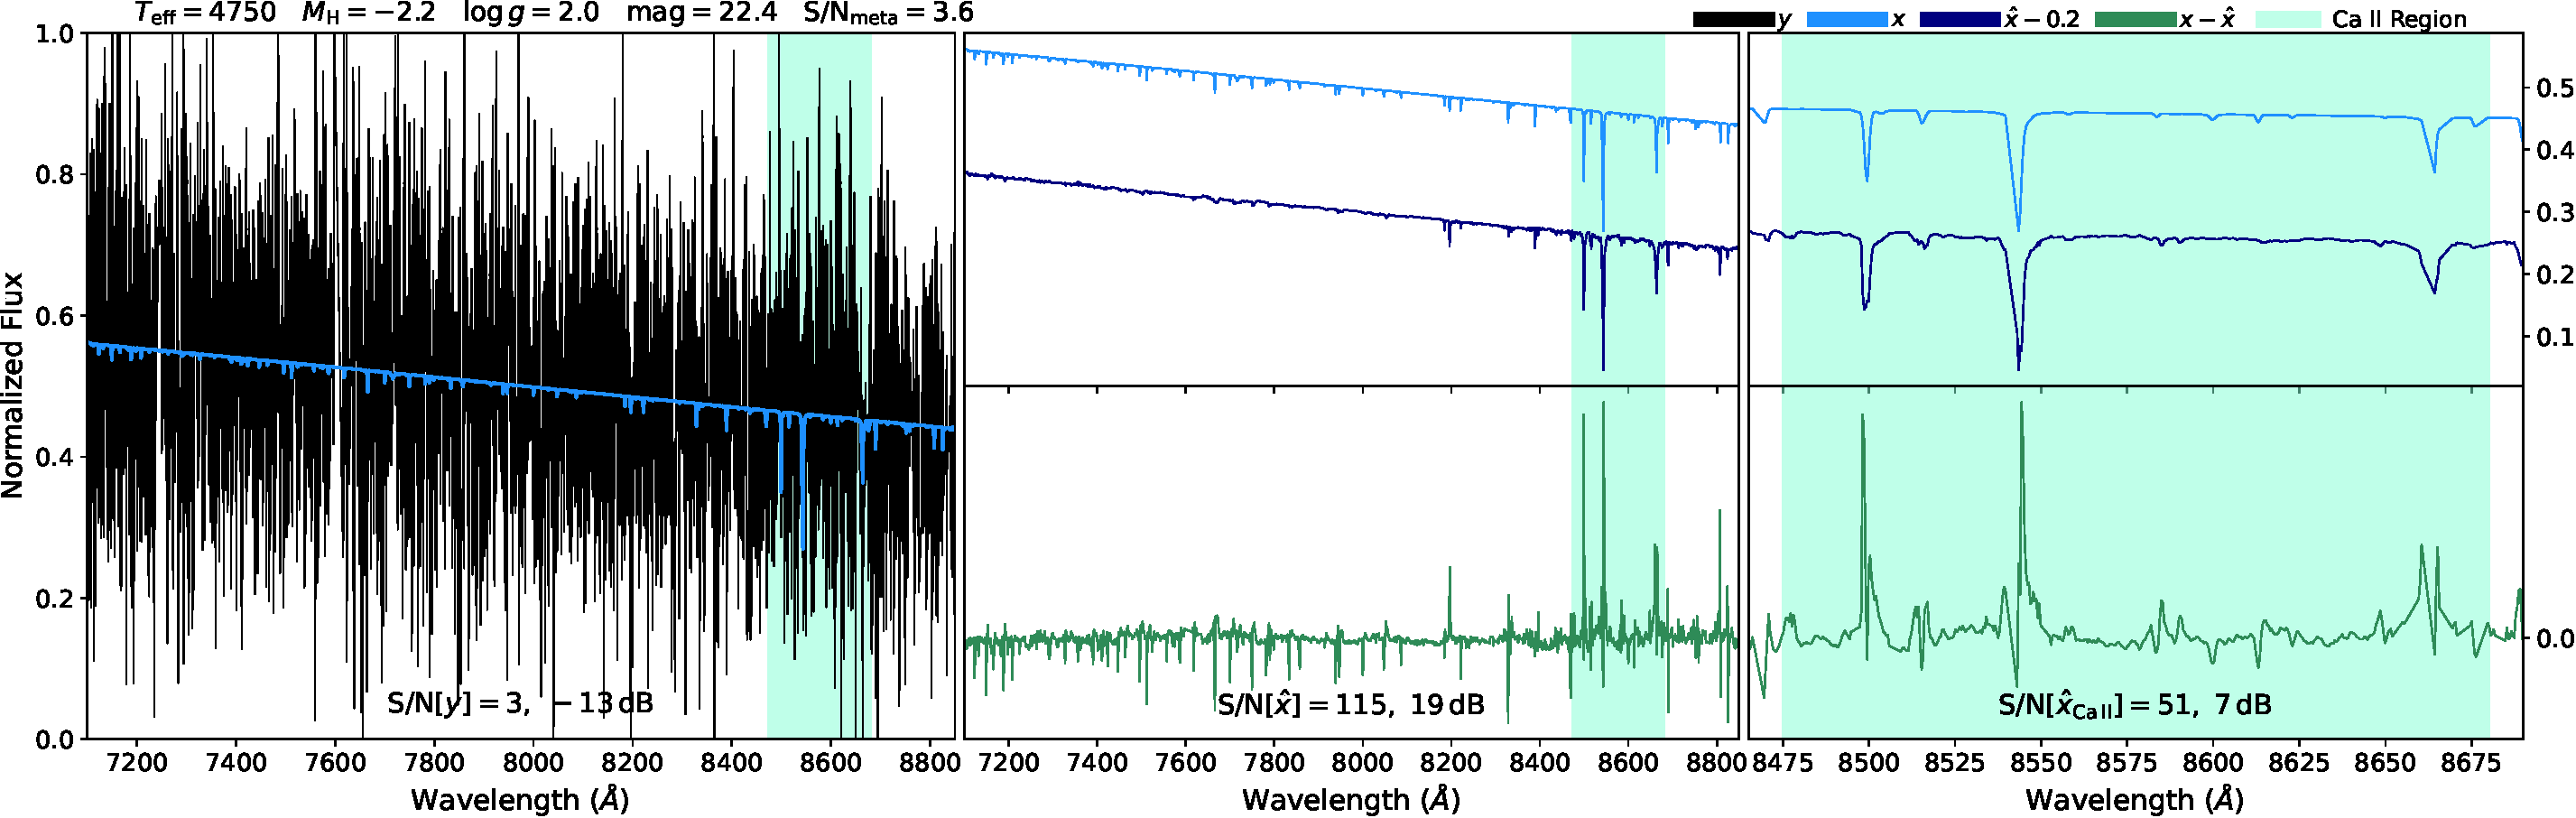
\includegraphics[width=\textwidth]{figs/fig1_representative.pdf}
\caption{Representative low-S/N test spectrum near the faint end of the magnitude range ($T_{\rm eff}=4750$~K, $\log g=2.0$, $[\mathrm{M}/\mathrm{H}]=-2.25$, $\mathrm{mag}=22.45$, input $\mathrm{S/N}[y]\approx3$). \textbf{Top:} noisy input $y$ and clean reference $x$ on the full mask-pruned wavelength grid, with the Ca\,\textsc{ii} triplet region shaded. \textbf{Middle:} clean reference $x$ and blindspot output $\hat{x}$, offset for readability, with the residual $x-\hat{x}$ shown below; this spectrum has $\mathrm{S/N}[\hat{x}]\approx115$. \textbf{Bottom:} Ca\,\textsc{ii} triplet zoom, where the line-restricted statistic is $\mathrm{S/N}[\hat{x}_{\rm Ca\,II}]\approx51$. The output follows the narrow Ca\,\textsc{ii} cores rather than flattening them toward the continuum.}
\label{fig:representative_spectrum}
\end{figure}

% ROLE: headline reconstruction comparison; full baseline ledger is in Appendix C.
\begin{table}[htbp]
\centering
\small
\caption{Test-set reconstruction quality on $10{,}000$ test spectra (mean and median per-spectrum reconstruction S/N, Equation~\ref{eq:snr_def}). Rows group the observed input, a validation-tuned clean-template PCA reference, the self-supervised blindspot with and without the scalar noise condition $\bar{\sigma}$, and a supervised clean-target reference. The clean-template PCA and supervised U-Net rows are fit with access to clean spectra and are not deployable comparisons; they bound the linear estimator class and the paired-data ceiling respectively. Baseline tuning grids and the noisy-trained PCA are listed in Appendix~\ref{app:controls_gamma}; the central-visible copy-shortcut control is in Appendix~\ref{app:architecture_integrity}.}
\label{tab:main_baselines}
\begin{tabular}{llcc}
\hline
Method & Reference type & Mean S/N & Median S/N [$5\%, 95\%$] \\
\hline
Noisy input & observed input & $7.6$ & $6.8$ [$3.1$, $14.6$] \\
PCA, $k\!=\!16$ (clean-template) & linear, clean reference & $55.7$ & $52.9$ [$27.1$, $93.0$] \\
Blindspot, no $\bar{\sigma}$ & self-supervised & $118$ & $104$ [$43$, $239$] \\
\textbf{Blindspot $+$ $\bar{\sigma}$ (ours)} & \textbf{self-supervised} & $\mathbf{122}$ & $\mathbf{109}$ [$\mathbf{45}$, $\mathbf{246}$] \\
Supervised U-Net & clean-target ceiling & $154$ & $136$ [$55$, $319$] \\
\hline
\end{tabular}
\end{table}

Table~\ref{tab:main_baselines} separates the deployable noisy-only estimator from non-deployable references. The central-visible copy control in Appendix~\ref{app:architecture_integrity} collapses to the noisy-input scale, so the gain depends on excluding the target bin rather than on same-input regression. The scalar noise condition is a small refinement, whereas the clean-template PCA result shows that access to noiseless training spectra does not by itself close the fixed-basis gap; Appendix~\ref{app:controls_gamma} records the full baseline ledger and the fixed-basis mechanism.

\subsection{Line-preservation diagnostics}
\label{sec:results_physical}

Aggregate reconstruction S/N does not by itself exclude simple smoothing or line filling. We therefore test the reconstructed spectra with two line-sensitive diagnostics --- relative equivalent-width error on each Ca\,\textsc{ii} triplet line and continuum-relative polarity flips --- and, separately, a high-noise control in the sky-dominated \mbox{O$_2$} A-band, which is an atmospheric-window stress test rather than a stellar-line diagnostic (Table~\ref{tab:main_results}).

% ROLE: compact main-text evidence against simple smoothing or line filling as the dominant explanation.
\begin{table}[htbp]
\centering
\small
\setlength{\tabcolsep}{5pt}
\caption{Line-sensitive reconstruction diagnostics on the test split. Equivalent-width entries use the relative error in Equation~\ref{eq:ew_relative_error}; polarity flips use Equation~\ref{eq:polarity_flip}. Per-line bootstrap confidence intervals, polarity subgroups, and the Ca\,\textsc{ii} morphology panel are reported in Appendix~\ref{app:line_addenda}.}
\label{tab:main_results}
\begin{tabular}{lcc}
\hline
Diagnostic & Noisy input $y$ & Blindspot output $\hat{x}$ \\
\hline
\multicolumn{3}{l}{\emph{Ca\,\textsc{ii} triplet relative EW error}} \\
$\quad 8498$~\AA{} & $0.737$ & $\mathbf{0.121}$ \\
$\quad 8542$~\AA{} & $0.328$ & $\mathbf{0.098}$ \\
$\quad 8662$~\AA{} & $1.02$ & $\mathbf{0.147}$ \\
\hline
\multicolumn{3}{l}{\emph{Continuum-relative polarity flips}} \\
$\quad$All non-continuum pixels & $0.276$ & $\mathbf{0.00302}$ \\
\hline
\multicolumn{3}{l}{\emph{\mbox{O$_2$} A-band window, $7590$--$7700$~\AA{}}} \\
$\quad$Window-restricted reconstruction S/N & $0.16$ & $\mathbf{3.6}$ \\
$\quad$Mean relative EW degradation & $22.2$ & $\mathbf{1.19}$ \\
\hline
\end{tabular}
\end{table}

The three diagnostic families point in the same direction: the recovery is not concentrated in a single Ca\,\textsc{ii} core, the local contrast usually returns to the clean spectrum's side of the continuum proxy, and the high-noise \mbox{O$_2$} window is not simply discarded under this simulator. Together with the morphology in Figures~\ref{fig:representative_spectrum} and~\ref{fig:caII_zoom}, these checks argue against generic smoothing as the explanation for the reconstruction gain.

\subsection{Downstream clean-trained calibrator transfer}
\label{sec:results_downstream_logg}

The final test asks whether the line-preserving reconstruction remains useful to an estimator trained only on clean spectra. Surface gravity carries the dwarf--giant separation that selects faint Galactic Archaeology samples; the downstream test therefore applies the full-spectrum $\log g$ calibrator of Section~\ref{sec:implementation}, without refitting, to clean references, blindspot outputs, noisy inputs, and a validation-tuned Savitzky--Golay smoother. The calibrator is evaluated on a disjoint $5{,}000$-spectrum BOSZ partition (Appendix~\ref{app:contract}); the clean-reference row is an upper reference under this fixed map, not a deployable comparison.

% ROLE: main fixed clean-trained gravity-transfer result.
\begin{table}[htbp]
\centering
\small
\caption{Clean-trained $\log g$ estimator on four reconstruction inputs, evaluated without refitting on $5{,}000$ test spectra. $\sigma_{\rm rob}$ is the centered Gaussian-equivalent dispersion of the residual $\widehat{\log g}-\log g_{\rm true}$; MAE and bias are the mean absolute and mean signed residuals; $R^{2}$ is the coefficient of determination. The clean-input row is an upper reference under the fixed mapping. Paired-bootstrap $95\%$ confidence intervals over $1000$ resamples on the blindspot-vs-noisy ratios are $\sigma_{\rm rob}$-ratio $0.64$ $[0.61,\,0.66]$ and MAE-ratio $0.70$ $[0.68,\,0.72]$.}
\label{tab:downstream_logg}
\begin{tabular}{lcccc}
\hline
Input spectrum & $\sigma_{\rm rob}$ [dex] & MAE [dex] & Bias [dex] & $R^{2}$ \\
\hline
Clean input (upper reference)         & $0.22$ & $0.20$ & $+0.001$ & $0.94$ \\
\textbf{Blindspot output (ours)}      & $\mathbf{0.80}$ & $\mathbf{0.67}$ & $\mathbf{+0.020}$ & $\mathbf{0.46}$ \\
Savitzky--Golay smoother (val.\ tuned)& $1.11$ & $0.88$ & $-0.078$ & $0.10$ \\
Noisy input                           & $1.26$ & $0.96$ & $-0.170$ & $0.01$ \\
\hline
\end{tabular}
\end{table}

The fixed map extracts gravity-discriminating information from clean inputs on this BOSZ support, and the blindspot output moves the same estimator away from the noisy-input regime across scatter, absolute error, bias, and $R^{2}$. The improvement remains short of the clean-reference row, so the result is a substantial transfer gain rather than full clean-domain recovery. Residual distributions, four-label context, and the calibrator train-size sweep are reported in Appendix~\ref{app:downstream_logg}.

\section{Discussion}
\label{sec:discussion}
The results form a three-step evidence chain. Noisy-only blindspot training first raises reconstruction S/N beyond the observed input and validation-tuned fixed-basis references. Line-sensitive diagnostics then show that this gain is not explained by simple continuum smoothing or line filling. Finally, a $\log g$ estimator trained only on clean spectra and evaluated without refitting reads more gravity-discriminating information from the blindspot output than from the noisy or conventionally smoothed inputs.

The claim is scoped to the independent zero-mean simulator of Section~\ref{sec:method}, with continuum-normalized late-type spectra and the PFS-like wavelength, resolution, and magnitude range of Table~\ref{tab:data_summary}. Real survey deployment introduces correlated sky-subtraction residuals, extraction covariance, varying line-spread functions, and continuum-estimation errors that are not tested here. Rest-frame alignment is also not a free baseline under the targeted noisy-only setting: it requires a velocity estimate or template assumption before resampling, and the fixed-basis saturation analyzed in Appendix~\ref{app:controls_gamma} shows why exact clean-template access is not equivalent to a deployable denoiser.

All main numerical results use one selected checkpoint and the evaluation protocol in Appendix~\ref{app:contract}. The reconstruction and line-preservation tables use one noise realization per test spectrum, while paired-bootstrap intervals resample spectra or downstream test examples as specified in the corresponding captions. The fixed-spectrum repeated-noise diagnostic in Appendix~\ref{app:noise_stability} measures sensitivity to noise draws for one clean spectrum; it is not uncertainty calibration, a training-seed robustness study, or evidence for all spectra.

The downstream result is estimator-specific. The clean-trained $\log g$ calibrator reads from the full flux vector and is never retrained on noisy or denoised spectra, so Table~\ref{tab:downstream_logg} tests transfer to that fixed surface-gravity estimator. It does not report a thresholded dwarf--giant confusion matrix, full stellar-label recovery, abundance preservation, or interchangeability with line-window fidelity scores that evaluate different functionals of the reconstruction.

\section{Conclusion}
\label{sec:conclusion}
On a continuum-normalized late-type BOSZ/PFS-like simulator with independent zero-mean per-pixel noise, a self-supervised blindspot denoiser trained only on noisy spectra delivers reconstructions that retain absorption-line structure and remain legible to a stellar-label estimator that never saw a noisy spectrum during its own training. The transfer is therefore not from one denoiser to a tuned downstream pipeline, but from a noisy-only training signal to a clean-trained scientific instrument used unchanged.

The claim is bounded to that simulator. Correlated sky-subtraction residuals, extraction covariance, drifting line-spread functions, and stellar regimes outside the faint late-type window are not part of what is shown.

\begin{acknowledgments}
This work is supported by the generosity of Eric and Wendy Schmidt, by recommendation of the Schmidt Futures program. We thank the developers and maintainers of the BOSZ synthetic stellar grid \citep{Bohlin2017} and of the underlying ATLAS9 model atmospheres \citep{Kurucz1979,Meszaros2012} that supply the clean templates used in every experiment, and the Subaru Prime Focus Spectrograph instrument team for the noise-model parameters used to set the simulated wavelength range, resolution, and per-pixel uncertainty profile. V.W. designed the experiments, implemented the blindspot architecture and training protocol, ran the test-set evaluation, the line-preservation diagnostics, the integrity audits, and the downstream calibrator transfer, and wrote the manuscript. L.D. provided the spectrum simulator and PFS-like noise configuration. A.S.S., T.B., and R.F.G.W. advised on the survey context and target metrics. X.Z. and B.P. contributed to discussions on the self-supervised denoising literature and on the evaluation design.
\end{acknowledgments}

\software{
    Astropy,
    LightGBM,
    NumPy,
    SciPy,
    Matplotlib,
    PyTorch
}

\appendix

\noindent The appendices are organized as follows. Appendix~\ref{app:contract} specifies the evaluation protocol and reproducibility contract. Appendix~\ref{app:architecture_integrity} documents the reported blindspot model and integrity audit. Appendix~\ref{app:controls_gamma} reports validation-tuned baselines and the consolidated method ledger. Appendix~\ref{app:context_recoverability} reports the context-recoverability measurements behind the small-$\gamma$ premise. Appendix~\ref{app:line_addenda} gives distributional reconstruction and line-preservation checks. Appendix~\ref{app:downstream_logg} reports downstream calibration checks. Appendix~\ref{app:noise_stability} reports fixed-spectrum repeated-noise stability.

\section{Evaluation Protocol and Reproducibility Contract}
\label{app:contract}

This appendix collects the evaluation protocol and reproducibility artifacts under which the numbers reported in Section~\ref{sec:results} and the supporting appendices are obtained: the public release that pins code and data, the canonical reconstruction split, the separate downstream-calibrator split, the rule that separates validation tuning from test-set evaluation, and the software environment. Apart from the trained-checkpoint row, this protocol is model-agnostic and is intended to be reusable for future denoisers evaluated on the same simulated support.

\paragraph{Archived release.}
The evaluation contract is defined by a versioned release bundle containing the trained checkpoint, evaluation script, downstream-calibrator script, simulator configuration, metric implementation, and per-baseline tuning record. Table~\ref{tab:contract_artifacts} lists the assets that define every quantitative result in the paper; each row names the release artifact that reproduces the corresponding paper table or figure panel.

% ROLE: reproducibility contract linking each quantitative claim to a release artifact.
\begin{table}[ht]
\centering
\small
\setlength{\tabcolsep}{4pt}
\caption{Artifacts defining the evaluation protocol. Each entry names an asset inside the versioned release bundle; the same release pins the selected checkpoint, the test split, and the metric implementation used for every quantitative result in this paper.}
\label{tab:contract_artifacts}
\begin{tabular}{lll}
\hline
Artifact & Role & Reproduces \\
\hline
Trained checkpoint & selected denoising model & Table~\ref{tab:main_baselines}, Table~\ref{tab:main_results}; Figs.~\ref{fig:representative_spectrum},~\ref{fig:caII_zoom},~\ref{fig:noise_ensemble} \\
Reconstruction test split & fixed reconstruction test set & Tables~\ref{tab:main_baselines},~\ref{tab:main_results}; Figs.~\ref{fig:representative_spectrum},~\ref{fig:caII_zoom} \\
Downstream calibrator split & clean-trained estimator evaluation & Table~\ref{tab:downstream_logg}; Fig.~\ref{fig:downstream_clean_domain_transfer} \\
Metric implementation & release-pinned metric code & all metric columns \\
Validation split + tuning record & per-baseline grids & Table~\ref{tab:main_baselines}, Table~\ref{tab:baseline_grids} \\
$\gamma$ predictor record & per-estimator measurements & Table~\ref{tab:gamma_main}, Table~\ref{tab:gamma_full} \\
Simulator configuration & noise model & Table~\ref{tab:data_summary} \\
Environment specification & software pin & all numerical results \\
\hline
\end{tabular}
\end{table}

\paragraph{Validation and test separation.}
The reconstruction training, validation, and test sets contain $200{,}000$, $1{,}000$, and $10{,}000$ spectra respectively, drawn without replacement from the same scope-restricted BOSZ library so that the marginal distributions over $T_{\rm eff}$, $\log g$, $[\mathrm{M}/\mathrm{H}]$, and magnitude match across splits. All hyperparameter selection --- the training-time validation rule for the blindspot model, the classical-baseline grids in Appendix~\ref{app:controls_gamma}, and the model-free $\gamma$ predictors --- uses the validation split alone, with a single fixed validation noise seed. After selection, the hyperparameters are held fixed, and the reconstruction and line-preservation results are computed on the reconstruction test split of $10{,}000$ spectra with one noise realization per spectrum. Reported intervals for the Ca\,\textsc{ii} equivalent-width rows are paired-bootstrap intervals over test spectra.

The downstream $\log g$ calibrator uses a separate labeled BOSZ pool of $50{,}000$ spectra. Calibrator training uses $30{,}000$ clean spectra; the fitted model is then evaluated without refitting on a disjoint $5{,}000$-spectrum test partition represented in four ways: clean reference, blindspot output, noisy input, and a Savitzky--Golay smoother. The blindspot-vs-noisy confidence intervals in Table~\ref{tab:downstream_logg} are paired-bootstrap intervals over $1000$ resamples of that $5{,}000$-spectrum downstream test partition.

\paragraph{Software environment.}
A dependency manifest and a container recipe are pinned in the archived release, so that the metric module, simulator, and inference script execute against the same software stack used to generate the reported numbers.

\section{Reported Model Configuration and Blindspot Integrity Audit}
\label{app:architecture_integrity}

This appendix is specific to the blindspot model and is not part of the model-agnostic evaluation contract of Appendix~\ref{app:contract}. It records the canonical model architecture and training configuration that produce the test-set reconstruction in Section~\ref{sec:results_denoising} and the numerical blindspot integrity audit that rules out leakage of $y_{\lambda}$ into $\hat{x}_{\lambda}$ in the reported network, in support of Section~\ref{sec:blindspot_algorithm} and the central-pixel exclusion claim in Section~\ref{sec:results_denoising}.

\paragraph{Canonical model and training configuration.}
The denoiser is a one-dimensional convolutional U-Net (Table~\ref{tab:training_config}) that maps a single-channel noisy spectrum, concatenated with the broadcast scalar $\bar{\sigma}$ as a second input channel, to a single-channel reconstruction $\hat{x}$. The backbone uses nine convolutional layers with width $48$ and kernel size $25$, batch normalization, and residual aggregation between matching encoder and decoder levels; the output is a single-head $\hat{x}$ point estimate, with no auxiliary $\sigma$ output head and no probabilistic output branch. The blindspot property is enforced by combining shifted causal convolutions on each side of the spectrum, as in Algorithm~\ref{alg:blindspot_forward}. Optimization uses Adam with $(\beta_1,\beta_2,\epsilon)=(0.9,0.999,10^{-8})$ and zero weight decay, initial learning rate $10^{-4}$, and a cosine schedule decaying to $10^{-6}$ over the full training horizon. Training uses $200$ epochs, batch size $128$, and a single fixed training seed; the early-stopping patience is $30$ epochs and the reported model is selected as the validation-best by reconstruction S/N before any test-set evaluation. At each training step, $85\%$ of wavelength bins are sampled at random and contribute to the noisy-target loss, while the remaining bins are held out from the loss for that step; this stochastic loss-mask is the standard blindspot-training mechanism for decorrelating successive predicted bins and does not modify the network input or the test-set evaluation, which is computed at every wavelength.

% ROLE: reproducibility record for the reported model checkpoint and training configuration.
\begin{table}[ht]
\centering
\small
\caption{Canonical blindspot model and training configuration used for all main-text and appendix results. The training-time loss-mask ratio is the random fraction of wavelength bins that contribute to the noisy-target loss at each step (the loss-mask trick); test-set evaluation is computed at every wavelength.}
\label{tab:training_config}
\begin{tabular}{ll}
\hline
\textbf{Quantity} & \textbf{Value} \\
\hline
Architecture & 1D shifted-causal blindspot U-Net \\
Convolutional layers & $9$ \\
Width & $48$ \\
Kernel size & $25$ \\
Normalization & batch normalization \\
Output head & single-channel $\hat{x}$ (no auxiliary $\sigma$ head) \\
Input channels & noisy spectrum + broadcast scalar $\bar{\sigma}$ \\
Loss & Huber, $\delta=0.03$ in normalized flux units \\
Training target & noisy observation \\
Optimizer & Adam, $(\beta_1,\beta_2,\epsilon)=(0.9,0.999,10^{-8})$ \\
Weight decay & $0$ \\
Initial learning rate & $10^{-4}$ \\
Learning-rate schedule & cosine decay to $10^{-6}$ \\
Batch size & $128$ \\
Epochs & $200$ \\
Early-stopping patience & $30$ epochs \\
Training-time loss-mask ratio & $0.85$ (per step, stochastic) \\
Training seed & $0$ (fixed) \\
Validation noise seed & fixed across training \\
Checkpoint selection rule & validation-best reconstruction S/N \\
\hline
\end{tabular}
\end{table}

\paragraph{Numerical blindspot integrity.}
The blindspot construction implies that $\hat{x}_{\lambda}$ depends on the input only through positions other than $\lambda$. We test this property numerically at three test-pixel positions, $i\in\{L/4, L/2, 3L/4\}$, on $64$ test spectra. For each spectrum and each position we forward the network on the noisy input and on a perturbed input that modifies $y_{i}$ but leaves $y_{j}$ unchanged for $j\neq i$, and record the central-pixel deviation $|\hat{x}^{\,\mathrm{perturbed}}_{i}-\hat{x}^{\,\mathrm{baseline}}_{i}|$. Two perturbations are reported: a cross-spectrum permutation in which $y_{i}$ is shuffled across the $64$ spectra, and a per-spectrum mean replacement in which $y_{i}$ is replaced by the spectrum-wise mean. Both perturbations leave the central output unchanged at the level reported in Table~\ref{tab:integrity_audit}, more than $400$ times below the $10^{-4}$ audit threshold, so the test-set gain in Section~\ref{sec:results_denoising} cannot be attributed to leakage of $y_{i}$ into $\hat{x}_{i}$.

% ROLE: reviewer defense that the reported blindspot output does not use the target pixel.
\begin{table}[ht]
\centering
\small
\caption{Blindspot integrity audit, where $\Delta := \hat{x}^{\,\mathrm{perturbed}}_{i}-\hat{x}^{\,\mathrm{baseline}}_{i}$ denotes the central-pixel deviation under perturbation. Each row reports $|\Delta|$ aggregated over three test-pixel positions and $64$ test spectra under a non-information-preserving perturbation of $y_{i}$. Both deviations are more than $400$ times below the $10^{-4}$ audit threshold.}
\label{tab:integrity_audit}
\begin{tabular}{lccc}
\hline
Perturbation of $y_{i}$ & Pixels tested & Spectra & Max $|\Delta|$ \\
\hline
Cross-spectrum permutation & $3$ & $64$ & $1.19\times10^{-7}$ \\
Per-spectrum mean replacement & $3$ & $64$ & $1.49\times10^{-7}$ \\
\hline
\end{tabular}
\end{table}

\paragraph{Central-visible copy-shortcut control.}
The blindspot and supervised rows of Table~\ref{tab:main_baselines} are paired with a training control that removes the blindspot exclusion. A variant of the same network that keeps the target bin $y_{\lambda}$ in its receptive field, trained against the same noisy target, learns to copy that bin: its test-split mean reconstruction S/N is $7.6$, the noisy-input scale, against $122$ for the blindspot. The collapse confirms that the reconstruction gain comes from excluding the target bin and not from ordinary same-input regression, complementing the architectural leakage audit above. The blindspot rows themselves are reported in Table~\ref{tab:main_baselines}: the scalar noise condition $\bar{\sigma}$ lifts the mean reconstruction S/N from $118$ to $122$, and the supervised clean-target U-Net reference reaches $154$.

\section{Validation-Tuned Baselines and Consolidated Method Ledger}
\label{app:controls_gamma}

This appendix records the validation grids for the non-neural reference methods of Table~\ref{tab:main_baselines}, the consolidated cross-method result ledger, and the fixed-basis explanation used to interpret the PCA-family baselines. Context-recoverability measurements are separated into Appendix~\ref{app:context_recoverability} so that baseline fairness and the small-$\gamma$ premise have distinct evidentiary roles.

\paragraph{Baseline tuning grids.}
Table~\ref{tab:baseline_grids} lists the validation grid searched for each non-neural reference method. Within each family the configuration that maximizes the linear-form reconstruction S/N of Equation~\ref{eq:snr_def} on the validation split at a fixed validation noise seed is the configuration evaluated on the test split in Table~\ref{tab:main_baselines} and Table~\ref{tab:appendix_baselines}; the same selection rule is applied to every family so the two test-split tables are internally comparable.

% ROLE: fair-comparison defense for validation-tuned non-neural baselines.
\begin{table}[ht]
\centering
\small
\setlength{\tabcolsep}{4pt}
\caption{Validation grids searched for the non-neural reference methods. The selection rule for every family is the validation-split reconstruction S/N maximizer at a fixed validation noise seed, before any test-set evaluation. The realized winning rank for the PCA-family rows is listed; the realized winning configurations for the smoother families correspond to the rows reported in Table~\ref{tab:main_baselines} (Wavelet BayesShrink) and Table~\ref{tab:appendix_baselines} (Savitzky--Golay, Gaussian smoothing, median filter).}
\label{tab:baseline_grids}
\begin{tabular}{lll}
\hline
Family & Grid searched & Selection rule \\
\hline
Savitzky--Golay & window $\in\{3,5,7,9,11\}$, order $\in\{1,2,3\}$ & validation S/N maximizer \\
Gaussian smoothing & $\sigma\in\{1,2,3,5,7\}$ pixels & validation S/N maximizer \\
Median filter & window $\in\{3,5,7\}$ pixels & validation S/N maximizer \\
Wavelet BayesShrink & db4, level $\in\{3,4,5\}$ & validation S/N maximizer \\
Noisy-PCA & $k\in\{16,32,64,128,256,512\}$, noisy-train fit & validation S/N maximizer ($k=16$) \\
Clean-template PCA reference & $k\in\{16,32,64,128\}$, clean-template fit & validation S/N maximizer ($k=16$) \\
\hline
\end{tabular}
\end{table}

\paragraph{Consolidated per-method results.}
Reconstruction signal-to-noise rises with estimator capacity, but the downstream $\log g$ estimator separates methods that preserve label information from those that only raise pixel S/N: the principal-component references reach the highest reconstruction S/N among the non-neural methods yet leave the calibrator no more accurate than the noisy input, whereas the blindspot moves the calibrator toward the clean-input scale.

% ROLE: single full cross-method ledger; other appendix tables should not duplicate this role.
\begin{table}[ht]
\centering
\footnotesize
\setlength{\tabcolsep}{4.5pt}
\caption{Consolidated per-method results on the matched-redshift test set ($z_1$; $10{,}000$ spectra). Reconstruction columns give the mean and median per-spectrum S/N (Equation~\ref{eq:snr_def}) with the $5$--$95\%$ range. The Ca\,\textsc{ii} EW column is the across-spectra mean of the per-spectrum triplet-averaged equivalent-width relative error; the polarity column is the continuum-relative flip rate. Robust per-line Ca\,\textsc{ii} medians with bootstrap intervals are in Table~\ref{tab:main_results}. The $\log g$ columns give the clean-trained calibrator residual scatter $\sigma_{\rm rob}$ (dex; smaller is better) and $R^2$, evaluated without refitting (Section~\ref{sec:results_downstream_logg}). Clean reference, clean-template PCA, and the supervised U-Net use clean data and are non-deployable; em-dashes mark quantities not computed for a row.}
\label{tab:appendix_baselines}
\begin{tabular}{lcccccc}
\hline
Method & Mean S/N & Median S/N [$5$,$95$] & Ca\,\textsc{ii} EW (mean) & Polarity & $\log g\ \sigma_{\rm rob}$ & $\log g\ R^2$ \\
\hline
Clean reference & --- & --- & --- & --- & $0.22$ & $0.94$ \\
Noisy input & $7.6$ & $6.8$ [$3.1$,$14.6$] & $3.09$ & $0.276$ & $1.26$ & $0.01$ \\
Savitzky--Golay & $20.8$ & $19.1$ [$9.7$,$38.2$] & $1.89$ & $0.121$ & $1.11$ & $0.10$ \\
Gaussian smoothing & $25.8$ & $23.1$ [$13.2$,$47.5$] & $1.49$ & $0.0842$ & $1.16$ & $0.05$ \\
Median filter & $15.7$ & $14.3$ [$6.7$,$29.1$] & $2.21$ & $0.168$ & $1.13$ & $0.04$ \\
Wavelet BayesShrink & $26.6$ & $24.2$ [$13.4$,$48.3$] & $1.50$ & $0.0804$ & $1.01$ & $0.13$ \\
Noisy-PCA, $k\!=\!16$ & $54.0$ & $51.0$ [$26.4$,$91.0$] & $1.09$ & $0.0184$ & $1.29$ & $-0.05$ \\
Clean-template PCA, $k\!=\!16$ & $55.7$ & $52.9$ [$27.1$,$93.0$] & $1.02$ & $0.0172$ & $1.28$ & $-0.05$ \\
\textbf{Blindspot (ours)} & $\mathbf{122}$ & $\mathbf{109}$ [$\mathbf{45}$,$\mathbf{246}$] & $\mathbf{0.51}$ & $\mathbf{0.003}$ & $\mathbf{0.80}$ & $\mathbf{0.46}$ \\
Supervised U-Net & $154$ & $136$ [$55$,$319$] & --- & --- & --- & --- \\
\hline
\end{tabular}
\end{table}

\paragraph{Why the fixed-basis linear estimators saturate.} The reconstruction ceiling of the principal-component baselines in Table~\ref{tab:appendix_baselines} is a property of the estimator class, not of how the basis was tuned. A fixed-grid linear basis must spend rank on two demands at once. Each spectrum carries a radial velocity of up to $\pm300$~km/s (Table~\ref{tab:data_summary}), which slides its absorption lines by several resolution elements, and representing an arbitrary shift on a fixed wavelength grid requires many Fourier modes rather than a few stellar-parameter directions. The narrow line cores are themselves high-frequency, low-variance features that again demand high rank. Both pressures push toward a large basis. Yet at the faint-end per-pixel S/N of this sample, every added component admits more noise variance than line variance, so the reconstruction-S/N-optimal rank is small: validation selects $k=16$ across the search range $\{16,\dots,512\}$. The linear class is therefore caught in a bias--variance bind, where the rank the signal structure demands is the rank the noise forbids, and no choice of rank --- with or without access to clean training targets --- escapes it. This is why the clean-template reference, fit on noiseless spectra, still reaches only $55.7$. Rest-frame alignment would add velocity-estimation and resampling assumptions rather than giving a free noisy-only baseline. The blindspot estimator is not a fixed-basis projection: it predicts each bin from the local shape of its neighborhood with the center withheld, so its accuracy is set by the physical correlation length of the signal relative to the per-bin noise (Section~\ref{sec:theory}) rather than by a global subspace dimension.

\section{Context-Recoverability Measurements}
\label{app:context_recoverability}

This appendix records the model-free measurements of the context-variance ratio $\gamma$ that operationalize the context-predictability premise of Section~\ref{sec:theory}. These measurements are a scope condition for interpreting the blindspot result, not a substitute for the reconstruction, line-preservation, or downstream tests in Section~\ref{sec:results}.

\paragraph{Compact context-recoverability summary.}
Table~\ref{tab:gamma_main} reports the conservative summaries used to check the small-$\gamma$ regime before the denoiser is evaluated.

% ROLE: compact support for the small-gamma recoverability premise.
\begin{table}[ht]
\centering
\small
\caption{Context-variance ratio $\gamma=\tau^2/\sigma^2$ on clean test spectra. The median-of-three row aggregates the three model-free predictors at each pixel by the per-pixel median; the worst-of-three row uses the per-pixel maximum across families and is the more conservative bound used by the small-$\gamma$ argument in Section~\ref{sec:theory}. The Ca\,\textsc{ii} $8542$~\AA{} column reports the line-core peak in each aggregation; the full per-estimator and per-line table is Table~\ref{tab:gamma_full}.}
\label{tab:gamma_main}
\begin{tabular}{lccc}
\hline
Aggregation & Median $\gamma$ & 95th pct.\ $\gamma$ & Ca\,\textsc{ii} $8542$~\AA{} \\
\hline
Median of three & $2.50\times10^{-5}$ & $8.80\times10^{-5}$ & $6.94\times10^{-4}$ \\
Worst of three families & $2.81\times10^{-4}$ & $1.00\times10^{-3}$ & $6.70\times10^{-3}$ \\
\hline
\end{tabular}
\end{table}

\paragraph{Heteroscedasticity and scalar $\gamma$.}
\label{app:gamma_heteroscedasticity}
The simulator draws $\epsilon_{\lambda}$ with the per-bin variance $\sigma_{\lambda}^{2}$ of Equation~\ref{eq:noise_components}, while the denoiser receives only the spectrum-level RMS noise condition $\bar{\sigma}$ of Equation~\ref{eq:blindspot_prediction}. The reported $\gamma$ values are therefore pixelwise residual-variance ratios summarized over wavelength, not a homoscedastic noise assumption. Windows whose variance profile differs from the spectrum-level summary are checked explicitly through the Ca\,\textsc{ii}, \mbox{O$_2$}, and TiO columns of Table~\ref{tab:gamma_full} and through the line-preservation diagnostics in Section~\ref{sec:results_physical}.

\paragraph{Risk interpretation of $\gamma$.}
\label{app:gamma_risk_interpretation}
The main text uses $\gamma$ only as a recoverability condition. In the local Gaussian model, the same ratio also gives the explicit comparison among three estimators of $x_{\lambda}$:
\[
    R_{\rm raw} = \sigma^{2},
    \qquad
    R_{\rm BS} = \tau^{2} = \gamma\,\sigma^{2},
    \qquad
    R_{\rm full} = \frac{\gamma}{1+\gamma}\,\sigma^{2}.
\]
The corresponding ratios are
\[
    \frac{R_{\rm raw}}{R_{\rm BS}} = \frac{1}{\gamma},
    \qquad
    \frac{R_{\rm BS}}{R_{\rm full}} = 1+\gamma,
    \qquad
    \frac{R_{\rm raw}}{R_{\rm full}} = 1 + \frac{1}{\gamma}.
\]
Thus, when $\gamma\ll1$, the context-only blindspot conditional-mean estimator is close to the center-visible conditional-mean estimator, while both are far better than leaving the noisy pixel unchanged. This calculation is only an interpretation of the measured context-residual ratio; it is not used as a substitute for the test-set reconstruction and line-preservation tests in Section~\ref{sec:results}.

\paragraph{Per-estimator $\gamma$ measurements.}
Table~\ref{tab:gamma_full} reports the model-free measurement of the context-variance ratio $\gamma=\tau^{2}/\sigma^{2}$ summarized in Table~\ref{tab:gamma_main}. The three predictor families and their tuned configurations are: local cubic interpolation (window radius $3$ pixels, selected over $\{3,5,8,16,32\}$); context-only PCA reconstruction with $k$ leading components (selected $k=256$ over $\{16,32,64,128,256\}$); and local ridge regression on a context Gaussian-process surrogate (window radius $32$ pixels, ridge regularization $\alpha=10^{-8}$, selected over a $5\times5$ grid of radius $\in\{3,5,8,16,32\}$ and $\alpha\in\{10^{-8},10^{-6},10^{-4},10^{-2},1\}$). Each family is tuned on the validation split by minimum residual variance and evaluated on the test split.

% ROLE: full per-estimator context-recoverability evidence for reviewer audit.
\begin{table}[ht]
\centering
\small
\caption{Model-free measurements of $\gamma=\tau^{2}/\sigma^{2}$ on clean test spectra. Ca\,\textsc{ii}, O$_2$, and TiO entries summarize the corresponding diagnostic windows. The median-of-three and worst-of-three rows are the aggregations promoted to the main-text Table~\ref{tab:gamma_main}.}
\label{tab:gamma_full}
\begin{tabular}{lccccc}
\hline
Predictor or aggregate & Median $\gamma$ & 95th pct.\ $\gamma$ & Ca\,\textsc{ii} 8542 & O$_2$ A-band & TiO 7650 \\
\hline
Local cubic interpolation & $6.37\times10^{-5}$ & $9.90\times10^{-4}$ & $6.70\times10^{-3}$ & $4.89\times10^{-5}$ & $9.01\times10^{-5}$ \\
Context-only PCA & $2.61\times10^{-4}$ & $5.75\times10^{-4}$ & $1.68\times10^{-3}$ & $1.84\times10^{-4}$ & $3.91\times10^{-4}$ \\
Local ridge regression & $9.32\times10^{-7}$ & $6.67\times10^{-5}$ & $3.35\times10^{-4}$ & $9.21\times10^{-7}$ & $1.22\times10^{-6}$ \\
Median of three & $2.50\times10^{-5}$ & $8.80\times10^{-5}$ & $6.94\times10^{-4}$ & $1.97\times10^{-5}$ & $2.60\times10^{-5}$ \\
Worst of three families & $2.81\times10^{-4}$ & $1.00\times10^{-3}$ & $6.70\times10^{-3}$ & $2.20\times10^{-4}$ & $3.91\times10^{-4}$ \\
\hline
\end{tabular}
\end{table}

\section{Distributional Reconstruction and Line-Preservation Checks}
\label{app:line_addenda}

This appendix checks that the reconstruction-S/N gain of Section~\ref{sec:results_denoising} and the line-preservation gain of Section~\ref{sec:results_physical} are distributed across the test-set input-S/N range and across diagnostic lines, rather than driven by a small subset of spectra. The polarity-flip threshold $0.02\,m_{s}$ is fixed across all rows of Table~\ref{tab:main_results} and Table~\ref{tab:appendix_baselines}; no alternative-threshold sweep is used in the claims.

\paragraph{Full line-sensitive diagnostics.}
Table~\ref{tab:main_results_full} is the full-precision version of the compact main-text line-preservation table. It preserves the exact polarity and bootstrap details while keeping the Results section within the main-text digit budget.

% ROLE: full-precision and bootstrap support for the compact main line-preservation table.
\begin{table}[htbp]
\centering
\footnotesize
\setlength{\tabcolsep}{4pt}
\caption{Full line-sensitive reconstruction diagnostics on the test split. Equivalent-width entries are per-spectrum medians of the relative error in Equation~\ref{eq:ew_relative_error}; bracketed intervals on the four Ca\,\textsc{ii} rows are $95\%$ paired-bootstrap confidence intervals from $1000$ resamples over the $10{,}000$ test spectra, where the same resample indices are applied to the noisy and denoised columns so the $\Delta$ interval captures per-spectrum correlation. The polarity rows count sign reversals relative to the per-spectrum continuum proxy in Equation~\ref{eq:polarity_flip}. The \mbox{O$_2$} A-band rows are included as a stress test in a high-noise atmospheric window, not as the main-text reconstruction result; bootstrap intervals are not reported on the polarity and \mbox{O$_2$} auxiliary rows.}
\label{tab:main_results_full}
\begin{tabular}{lccc}
\hline
 & \textbf{Noisy input $y$} & \textbf{Blindspot output $\hat{x}$} & \textbf{$\Delta=\hat{x}-y$} \\
\hline
\multicolumn{4}{l}{\emph{Ca\,\textsc{ii} triplet relative EW error}} \\
$\quad 8498$~\AA   & $0.737$ [$0.709$, $0.764$] & $\mathbf{0.121}$ [$\mathbf{0.117}$, $\mathbf{0.126}$] & $-0.616$ [$-0.641$, $-0.590$] \\
$\quad 8542$~\AA   & $0.328$ [$0.318$, $0.339$] & $\mathbf{0.098}$ [$\mathbf{0.095}$, $\mathbf{0.101}$] & $-0.230$ [$-0.241$, $-0.220$] \\
$\quad 8662$~\AA   & $1.02$ [$0.983$, $1.066$] & $\mathbf{0.147}$ [$\mathbf{0.142}$, $\mathbf{0.151}$] & $-0.873$ [$-0.919$, $-0.838$] \\
$\quad$Triplet mean & $0.695$ [$0.676$, $0.718$] & $\mathbf{0.122}$ [$\mathbf{0.119}$, $\mathbf{0.125}$] & $-0.573$ [$-0.595$, $-0.555$] \\
\hline
\multicolumn{4}{l}{\emph{Polarity-flip rate against the per-spectrum continuum median}} \\
$\quad$All non-continuum pixels                 & $0.276$ & $\mathbf{0.00302}$ & $-0.273$ \\
$\quad$Below-continuum pixels ($x<m$)           & $0.270$ & $\mathbf{0.00362}$ & $-0.266$ \\
$\quad$Above-continuum pixels ($x>m$)           & $0.282$ & $\mathbf{0.00242}$ & $-0.280$ \\
\hline
\multicolumn{4}{l}{\emph{Telluric \mbox{O$_2$} A-band hard window ($7590$--$7700$~\AA, $181$ pixels)}} \\
$\quad$Window-restricted S/N, linear & $0.16$ & $\mathbf{3.6}$ & $+3.4$ \\
$\quad$Mean relative EW degradation       & $22.2$ & $\mathbf{1.19}$ & $-21.0$ \\
\hline
\end{tabular}
\end{table}

% ROLE: morphology check that the line-preservation table is not only an aggregate metric effect.
\begin{figure}[htbp]
\centering
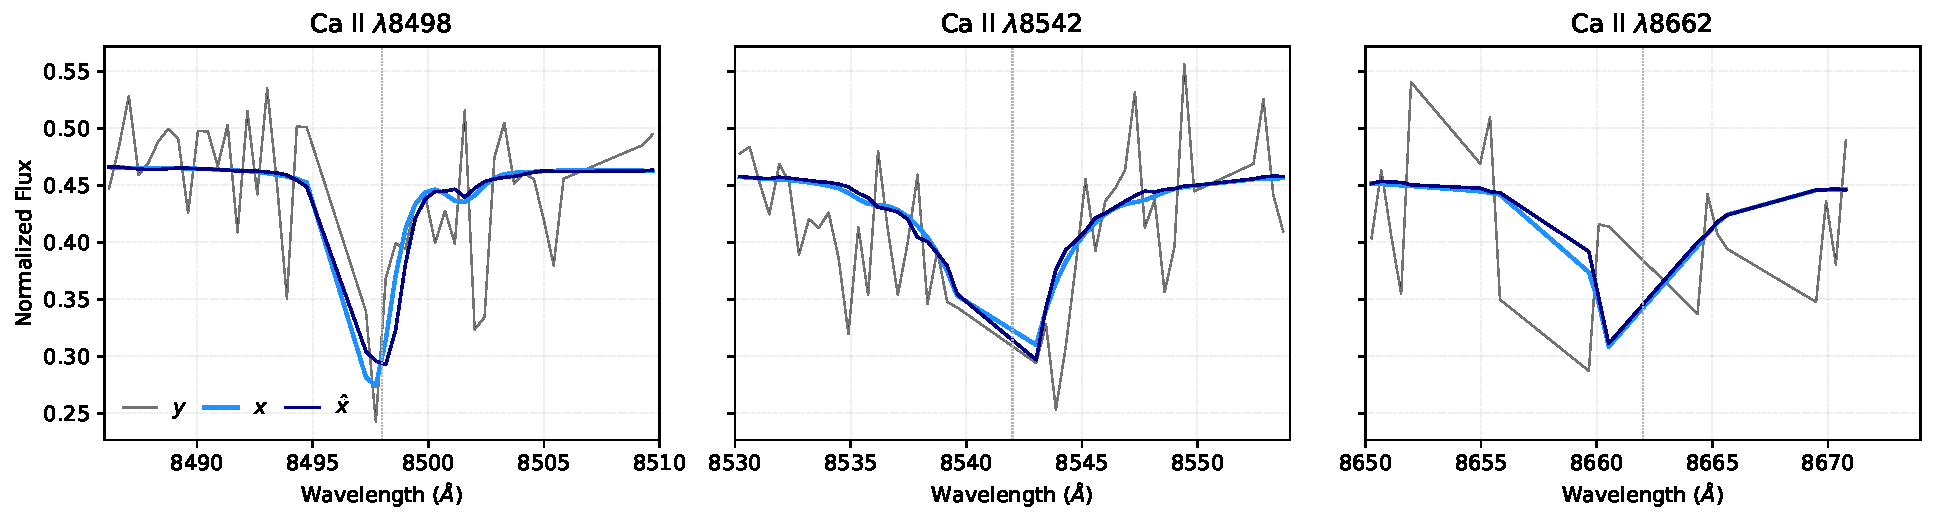
\includegraphics[width=\linewidth]{figs/fig3_caII_zoom_panels.pdf}
\caption{Ca\,\textsc{ii} triplet zoom for the same representative test spectrum as Figure~\ref{fig:representative_spectrum}. The panels show the $8498$, $8542$, and $8662$~\AA{} lines. Each panel overlays the noisy input $y$, the clean reference $x$, and the blindspot output $\hat{x}$. Markers indicate the individual sampled wavelength bins; connecting lines are visual guides only. In the $8542$~\AA{} panel, the apparent asymmetry of the clean reference is caused by the mask-pruned wavelength sampling around the line center, not by an asymmetric input line model. The blindspot reconstruction follows the depth and width of the Ca\,\textsc{ii} cores without flattening them toward the continuum.}
\label{fig:caII_zoom}
\end{figure}

% ROLE: distributional robustness of reconstruction S/N across input S/N.
\begin{figure}[ht]
\centering
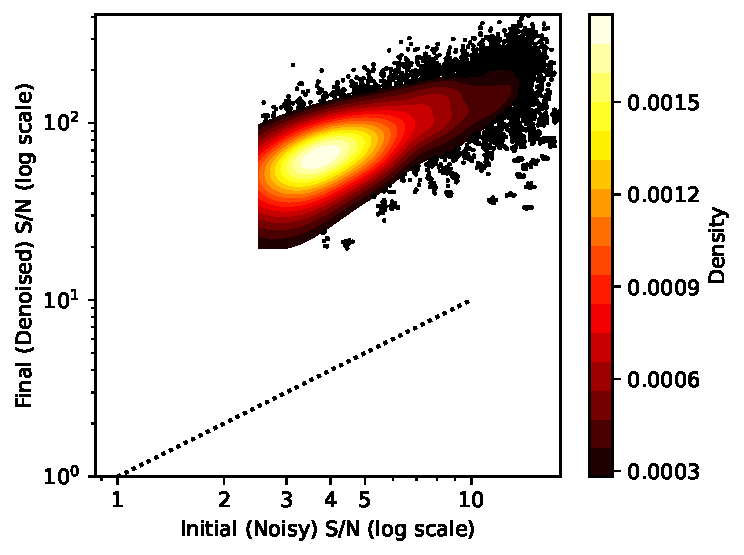
\includegraphics[width=0.6\linewidth]{figs/appendix/fig_snr_improvement_log.pdf}
\caption{Joint density of per-spectrum input (noisy) and output (denoised) signal-to-noise ratio on the test set, on log--log axes. The two-dimensional density (hot colormap; KDE) is overlaid with low-density outliers as black points; the dotted diagonal marks the $y{=}x$ identity. The bulk lies above the diagonal across the full input-S/N decade, so the reconstruction gain is approximately log-uniform in input S/N rather than driven by any single S/N range.}
\label{fig:appendix_snr_panel}
\end{figure}

% ROLE: distributional robustness of EW preservation across diagnostic lines and input S/N.
\begin{figure}[ht]
\centering
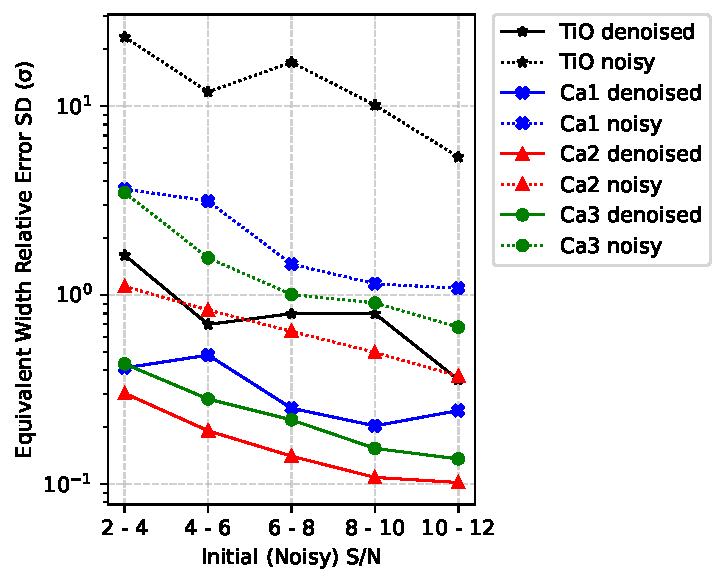
\includegraphics[width=0.6\linewidth]{figs/appendix/fig_ew_residual_std.pdf}
\caption{Equivalent-width preservation across diagnostic lines and input S/N. Standard deviation of the EW relative error as a function of input S/N for the TiO band near $7650$~\AA{} and the three Ca\,\textsc{ii} triplet lines (solid: denoised; dotted: noisy). The denoised dispersion is reduced by an order of magnitude in the lowest-S/N bin and the gain narrows monotonically as input S/N rises, so the recovery is most useful where the noisy measurement is least informative; lines with intrinsically larger EW recover more cleanly than the weaker TiO band, consistent with line strength governing recoverability.}
\label{fig:appendix_ew_panel}
\end{figure}

Figure~\ref{fig:appendix_snr_panel} resolves the test-set aggregate reconstruction S/N of Section~\ref{sec:results_denoising} into the joint distribution of per-spectrum input and output values, while Figure~\ref{fig:appendix_ew_panel} resolves the line-preservation result of Section~\ref{sec:results_physical} into the dispersion of the EW relative error across diagnostic features as input S/N varies. Together they show that neither the S/N gain nor the EW-error reduction is dominated by a narrow input-S/N subset: the input--output S/N density lies above the identity across the full input-S/N decade, and the dispersion of the EW relative error after denoising is reduced over the entire diagnostic feature set rather than for a single Ca\,\textsc{ii} core or a single S/N bin.

\section{Clean-Trained Gravity Calibrator Checks}
\label{app:downstream_logg}

This appendix provides the downstream residual visualizations and train-size stability check referenced in Section~\ref{sec:results_downstream_logg}. The main downstream claim remains the fixed clean-trained $\log g$ result in Table~\ref{tab:downstream_logg}; the auxiliary panels here check residual shape, split-seed stability, and whether the same ordering is tied to a single calibrator-training size.

% ROLE: downstream residual visualization and auxiliary four-label context; not a full all-label recovery claim.
\begin{figure}[htbp]
\centering
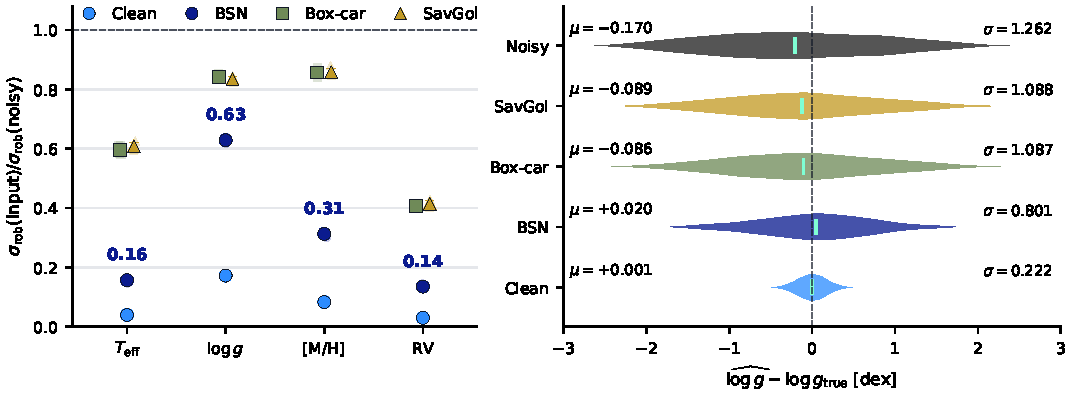
\includegraphics[width=\textwidth]{figs/fig4_downstream_clean_domain_transfer.pdf}
\caption{Clean-trained downstream calibration after denoising. Full-spectrum LightGBM calibrators are trained only on clean spectra and then evaluated, without refitting, on the same test spectra represented as clean inputs, blindspot outputs, Savitzky--Golay smooths, or noisy inputs. \textbf{Left:} centered robust-scatter ratio relative to the noisy input at $n_{\rm train}=30{,}000$ for four BOSZ labels; small points are five random splits, large markers are split means, and bars are split standard deviations. \textbf{Right:} residual distributions for the $\log g$ evaluation on the $5{,}000$-spectrum test partition in Table~\ref{tab:downstream_logg}. Side labels report $\mu$ (mean bias) and $\sigma$ (centered robust scatter) in dex.}
\label{fig:downstream_clean_domain_transfer}
\end{figure}

The four-label panel is an auxiliary consistency check under the same clean-trained transfer protocol; it is not used to claim full stellar-label recovery. The $\log g$ residual panel is the visual companion to the main downstream table.

The same clean-trained gradient-boosted regressor is refit at four training-size operating points, holding the test split and evaluation protocol fixed; only the calibrator's training-size hyperparameter changes between rows (Table~\ref{tab:downstream_logg_sweep}).

% ROLE: robustness check that the logg transfer result is not a single training-size artifact.
\begin{table}[ht]
\centering
\small
\caption{Train-size stability of the $\log g$ calibrator. Each entry is the centered robust scatter $\sigma_{\rm rob}$ [dex] of the residual $\widehat{\log g}-\log g_{\rm true}$ on the same $5{,}000$-spectrum test set used in Table~\ref{tab:downstream_logg}. Smaller is better. The clean-input column improves monotonically with calibrator-training size, while the noisy and smoothed columns stay near the noisy-input scale; the blindspot column stays closer to the clean column than the noisy or smoothed columns at every training size, though its gap to the clean column widens as the clean column improves.}
\label{tab:downstream_logg_sweep}
\begin{tabular}{rcccc}
\hline
$n_{\rm train}$ & Clean & Blindspot & Savitzky--Golay & Noisy \\
\hline
$1{,}000$  & $0.68$ & $1.02$ & $1.12$ & $1.32$ \\
$3{,}000$  & $0.39$ & $0.90$ & $1.10$ & $1.29$ \\
$10{,}000$ & $0.27$ & $0.83$ & $1.09$ & $1.28$ \\
$30{,}000$ & $0.22$ & $0.80$ & $1.11$ & $1.26$ \\
\hline
\end{tabular}
\end{table}

The sweep is consistent with stable clean-domain transfer at degraded fidelity: the blindspot column tracks the clean column more closely than the noisy or smoothed columns as the calibrator training size changes. This rules out the narrower reading that the gain in Table~\ref{tab:downstream_logg} is a special feature of the maximum-training-size operating point.

\section{Fixed-Spectrum Repeated-Noise Stability}
\label{app:noise_stability}

This appendix records the repeated-noise diagnostic referenced from Section~\ref{sec:results_downstream_logg} and from the reproducibility scope paragraph of Section~\ref{sec:discussion}. The main-text reconstruction and downstream calibration use one selected trained model; we test whether the reported point estimates are stable to repeated noise perturbations of a fixed clean spectrum. Holding one test clean spectrum $x$ fixed, we draw $10^{4}$ independent noise realizations from the same heteroscedastic simulator, denoise each realization, and summarize the output ensemble by its mean $\langle\hat{x}\rangle$ and across-draw spread $\sigma_{\hat{x}}$.

% ROLE: fixed-spectrum noise-draw stability only; not uncertainty calibration or training-seed robustness.
\begin{figure}[htbp]
\centering
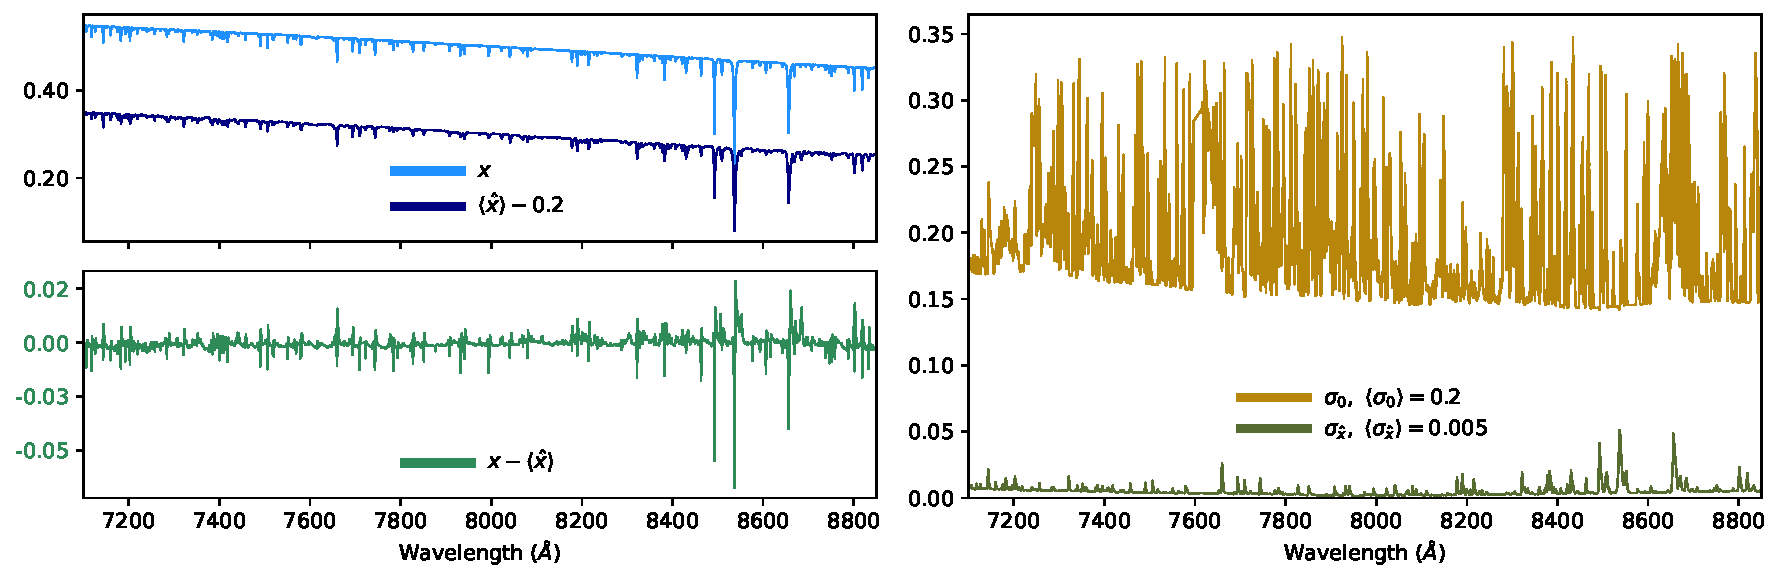
\includegraphics[width=\linewidth]{figs/fig2_noise_ensemble.pdf}
\caption{Fixed-spectrum repeated-noise diagnostic for the reported blindspot model. One clean test spectrum is perturbed by $10^{4}$ independent noise draws and denoised repeatedly. \textbf{Top-left:} clean spectrum $x$ and repeated-draw mean estimate $\langle \hat{x} \rangle$, shifted for readability. \textbf{Bottom-left:} residual $x-\langle \hat{x} \rangle$. \textbf{Right:} input noise scale and across-draw spread $\sigma_{\hat{x}}$ of the denoised outputs on a shared linear axis. This diagnostic measures sensitivity to noise realizations for a fixed spectrum; it is not a calibrated uncertainty estimate.}
\label{fig:noise_ensemble}
\end{figure}

Figure~\ref{fig:noise_ensemble} shows that the repeated-draw mean follows the clean spectrum and that the denoised spread remains far below the input noise scale over most wavelengths for this fixed spectrum. The diagnostic supports stability to repeated simulator noise draws in this example only; it should not be read as posterior uncertainty calibration, an error bar on individual line measurements, population robustness, or robustness to all training seeds.

\bibliographystyle{aasjournalv7}
\bibliography{cas-refs.cleaned}

\end{document}
